% This must be in the first 5 lines to tell arXiv to use pdfLaTeX, which is strongly recommended.
\pdfoutput=1
% In particular, the hyperref package requires pdfLaTeX in order to break URLs across lines.

\documentclass[11pt]{article}

% Change "review" to "final" to generate the final (sometimes called camera-ready) version.
% Change to "preprint" to generate a non-anonymous version with page numbers.
\usepackage[preprint]{acl}

% Standard package includes

\usepackage{longtable}
\usepackage{anyfontsize}
\usepackage{multicol}
\usepackage{lmodern}
\usepackage{relsize}
\usepackage{multirow}
\usepackage{afterpage}
\usepackage{times}
\usepackage{latexsym}
\usepackage{amssymb}
\usepackage{pifont}
\usepackage{tikz}
\usepackage{comment}
\usepackage{tcolorbox}
\tcbuselibrary{listingsutf8}

\usetikzlibrary{shapes, arrows.meta, positioning, backgrounds}

\newcommand{\cmark}{\ding{51}}%
\newcommand{\xmark}{\ding{55}}%


% For proper rendering and hyphenation of words containing Latin characters (including in bib files)
\usepackage[T1]{fontenc}
% For Vietnamese characters
% \usepackage[T5]{fontenc}
% See https://www.latex-project.org/help/documentation/encguide.pdf for other character sets

% This assumes your files are encoded as UTF8
\usepackage[utf8]{inputenc}

% This is not strictly necessary, and may be commented out,
% but it will improve the layout of the manuscript,
% and will typically save some space.
\usepackage{microtype}
\usepackage{amsmath} 
\definecolor{darkgreen}{rgb}{0.0, 0.7, 0.0}

% This is also not strictly necessary, and may be commented out.
% However, it will improve the aesthetics of text in
% the typewriter font.
\usepackage{inconsolata}

%Including images in your LaTeX document requires adding
%additional package(s)
\usepackage{graphicx}
\usepackage{xcolor}
\usepackage{booktabs}


% If the title and author information does not fit in the area allocated, uncomment the following
%
%\setlength\titlebox{<dim>}
%
% and set <dim> to something 5cm or larger.

\title{\raisebox{-0.1cm}{
\includegraphics[width=0.8cm,height=0.8cm,keepaspectratio]{pictures/coral.jpg}}CORAL: Benchmarking Multi-turn Conversational Retrieval-Augmentation Generation}

%\title{CORAL: Benchmarking Multi-turn Conversational Retrieval-Augmentation Generation}

% Author information can be set in various styles:
% For several authors from the same institution:
% \author{Author 1 \and ... \and Author n \\
%         Address line \\ ... \\ Address line}
% if the names do not fit well on one line use
%         Author 1 \\ {\bf Author 2} \\ ... \\ {\bf Author n} \\
% For authors from different institutions:
% \author{Author 1 \\ Address line \\  ... \\ Address line
%         \And  ... \And
%         Author n \\ Address line \\ ... \\ Address line}
% To start a separate ``row'' of authors use \AND, as in
%\author{Author 1 \\ Address line \\  ... \\ Address line
%        \AND
%        Author 2 \\ Address line \\ ... \\ Address line %\And         Author 3 \\ Address line \\ ... \\ Address % line}





\author{Yiruo Cheng$^1$, Kelong Mao$^1$, Ziliang Zhao$^1$, Guanting Dong$^1$, Hongjin Qian$^2$, \\
{\bf Yongkang Wu$^3$,} {\bf Tetsuya Sakai$^4$,} {\bf Ji-Rong Wen$^1$,} {\bf Zhicheng Dou$^1$}\thanks{Corresponding author.}
\\
$^1$Gaoling School of Artificial Intelligence, Renmin University of China \\
$^2$Beijing Academy of Artificial Intelligence \\
$^3$Huawei Poisson Lab\\
$^4$Waseda University, Tokyo, Japan \\
\texttt{\{chengyr,mkl,dou\}@ruc.edu.cn}  }

%\author{
%  \textbf{First Author\textsuperscript{1}},
%  \textbf{Second Author\textsuperscript{1,2}},
%  \textbf{Third T. Author\textsuperscript{1}},
%  \textbf{Fourth Author\textsuperscript{1}},
%\\
%  \textbf{Fifth Author\textsuperscript{1,2}},
%  \textbf{Sixth Author\textsuperscript{1}},
%  \textbf{Seventh Author\textsuperscript{1}},
%  \textbf{Eighth Author \textsuperscript{1,2,3,4}},
%\\
%  \textbf{Ninth Author\textsuperscript{1}},
%  \textbf{Tenth Author\textsuperscript{1}},
%  \textbf{Eleventh E. Author\textsuperscript{1,2,3,4,5}},
%  \textbf{Twelfth Author\textsuperscript{1}},
%\\
%  \textbf{Thirteenth Author\textsuperscript{3}},
%  \textbf{Fourteenth F. Author\textsuperscript{2,4}},
%  \textbf{Fifteenth Author\textsuperscript{1}},
%  \textbf{Sixteenth Author\textsuperscript{1}},
%\\
%  \textbf{Seventeenth S. Author\textsuperscript{4,5}},
%  \textbf{Eighteenth Author\textsuperscript{3,4}},
%  \textbf{Nineteenth N. Author\textsuperscript{2,5}},
%  \textbf{Twentieth Author\textsuperscript{1}}
%\\
%\\
%  \textsuperscript{1}Affiliation 1,
%  \textsuperscript{2}Affiliation 2,
%  \textsuperscript{3}Affiliation 3,
%  \textsuperscript{4}Affiliation 4,
%  \textsuperscript{5}Affiliation 5
%\\
%  \small{
%    \textbf{Correspondence:} \href{mailto:email@domain}{email@domain}
%  }
%}

\begin{document}
\maketitle
\begin{abstract}
Retrieval-Augmented Generation (RAG) has become a powerful paradigm for enhancing large language models (LLMs) through external knowledge retrieval. Despite its widespread attention, existing academic research predominantly focuses on single-turn RAG, leaving a significant gap in addressing the complexities of multi-turn conversations found in real-world applications. To bridge this gap, we introduce CORAL, a large-scale benchmark designed to assess RAG systems in realistic multi-turn conversational settings. CORAL includes diverse information-seeking conversations automatically derived from Wikipedia and tackles key challenges such as open-domain coverage, knowledge intensity, free-form responses, and topic shifts. It supports three core tasks of conversational RAG: passage retrieval, response generation, and citation labeling. We propose a unified framework to standardize various conversational RAG methods and conduct a comprehensive evaluation of these methods on CORAL, demonstrating substantial opportunities for improving existing approaches. Our dataset and code are available at \url{https://github.com/Ariya12138/CORAL}.
% Conversational Retrieval-Augmented Generation (RAG) integrates large language models with external knowledge retrieval to enhance question-answering accuracy in multi-turn conversations. However, a significant limitation in this emerging field is the lack of high-quality datasets for benchmarking various methods. To address this, we introduce CORAL, a benchmark dataset specifically designed for evaluating multi-turn conversational RAG methods. CORAL consists of four types of dialogue structures with 8,000 conversations, each of which features logical relationships between turns and citation labeling in responses. Our evaluation metrics focus on retrieval accuracy, generation quality, and citation performance, providing a comprehensive framework for assessing conversational RAG systems. Our dataset and code are available at \href{https://anonymous.4open.science/r/CORAL-08E3}{this repository}.
\end{abstract}

\section{Introduction}\label{introduction} 
Retrieval-Augmented Generation (RAG) has emerged as a promising approach in question answering, leveraging large language models (LLMs) alongside external knowledge retrieval to enhance the quality and accuracy of generated responses~\citep{Lewis_nips20_rag,guu_realm,huang_rag_survey}. While RAG has gained traction both in academia and industry, a notable gap exists between how it is studied in academic settings and how it is implemented in real-world systems. Academic research predominantly focuses on single-turn interactions~\citep{tan_acl24_simplm,jin_acl24_bider,wang_richrag,dong2024toward,zhu_spring}, whereas most industrial RAG systems~\cite{chatgpt,claude,kimichat,doubao} are designed to handle multi-turn conversations. In practice, multi-turn conversation is the norm, where RAG systems must dynamically adapt to evolving context and user intent across multiple turns.

The shift from single-turn to multi-turn conversations introduces unique challenges for RAG. In multi-turn settings, systems must deal with redundant or irrelevant information from prior interactions and cope with abrupt topic shifts~\citep{ye_sigir24_convrag,topiocqa}. This complexity can degrade the retrieval and generation quality, especially as conversation histories grow, exacerbating the ``long context problem''~\citep{Ratner_ACL23_PCW,LongRoPE}. These issues highlight the need for dedicated research into multi-turn conversational RAG to address the realities of interactive, ongoing dialogue.


\begin{table*}
\centering
\setlength{\tabcolsep}{2.8pt} % Reduce space between columns
\footnotesize % Smaller than \small
\scalebox{0.9}{
\begin{tabular}{lccccc}

\toprule
\textbf{Dataset} & \textbf{Open-domain} & \textbf{Knowledge-Intensive} & \textbf{Free-form Response} & \textbf{Topic Shift} & \textbf{Citation Labeling}\\ 
\midrule
CORAL (ours) & \cmark & \cmark & \cmark & \cmark & \cmark \\ 
\midrule
TopiOCQA~\citep{topiocqa} & \cmark & \cmark & \cmark & \cmark & \xmark \\ 
QReCC~\citep{Anantha_naacl21_cqr} & \cmark & \cmark & \cmark & \xmark & \xmark \\ 
Wizard of Wikipedia~\citep{wizard_of_wikipedia} & \cmark & \cmark & \cmark & \xmark & \xmark \\
CoQA~\citep{reddy2019coqa} & \xmark & \cmark & \cmark & \xmark & \xmark \\
OR-QuAC~\citep{or_quac} & \cmark & \cmark & \xmark & \xmark & \xmark \\

Doc2Dial~\citep{doc2dial} & \xmark & $\bigtriangleup$ & \cmark & \xmark & \xmark \\
TREC CAsT19~\citep{cast19} & \cmark & \cmark & \xmark & \xmark & \xmark \\
TREC CAsT20~\citep{cast20} & \cmark & \cmark & \cmark & \cmark & \xmark \\
TREC CAsT21~\citep{cast21} & \cmark & \cmark & \cmark & \cmark & \xmark \\
TREC CAsT22~\citep{cast22} & \cmark & \cmark & \cmark & \cmark & \xmark \\
\bottomrule
\end{tabular} }
\caption{Comparison of CORAL with other conversational search and conversational QA datasets. $\bigtriangleup$ indicates that only a portion of the dataset satisfies the property.}
\label{tab:dataset_comparison}
\end{table*}

However, progress in this area is severely hindered by the lack of a comprehensive benchmark designed to evaluate conversational RAG systems.
To align with the diverse and complex real-world applications of conversational RAG systems, we identify several critical features such a benchmark should satisfy: (1) open-domain coverage, allowing the system to handle questions from a wide range of topics; (2) knowledge-intensiveness, challenging systems to retrieve and generate responses that require deep, contextual knowledge; (3) free-form response generation, ensuring that models can produce detailed, contextually rich answers; (4) handling of topic shifts, evaluating the system’s ability to manage sudden changes in dialogue context without carrying over irrelevant information from previous turns; and (5) citation labeling, promoting transparency by requiring the system to cite the sources of the information it retrieves.

% However, before addressing these challenges, a more fundamental issue arises: the lack of a high-quality benchmark specifically designed to evaluate and compare different conversational RAG methods.
% Although there are numerous datasets for conversational search and conversational QA, they have significant limitations. 
% For instance, the conversational search dataset TREC CAsT19~\citep{cast19} is designed for conversation-based retrieval tasks but lacks free-form answers. Subsequent datasets such as TREC CAsT20~\citep{cast20}, TREC CAsT21~\citep{cast21}, and TREC CAsT22~\citep{cast22} begin to focus on answer generation but continue to be hindered by inadequate data volumes and limited dialogue scenarios. Additionally, conversational QA datasets such as QReCC~\citep{Anantha_naacl21_cqr} and TopiOCQA~\citep{topiocqa} mainly provide short answers without citation labeling and lack long-form responses, which are often observed in real-world scenarios.
% More importantly, these datasets fail to concentrate on the core challenges presented by conversational RAG: redundant information and the long window problem introduced by the conversation history.
% The absence of a high-quality conversational RAG benchmark hinders the systematic assessment and advancement of RAG techniques in this emerging area.

Unfortunately, no existing dataset satisfies all of these features.
Although there are datasets for related tasks, such as conversational search and question answering, they do not adequately address the unique challenges of benchmarking multi-turn conversational RAG systems that align with all of the above features. For instance, datasets in conversational search like TREC CAsT~\citep{cast19,cast20,cast21,cast22} primarily focus on retrieval tasks and lack the capacity to assess a system's generative abilities in producing free-form answers. Likewise, conversational QA datasets, such as QReCC~\citep{Anantha_naacl21_cqr} and TopiOCQA~\citep{topiocqa}, predominantly offer short, factual answers, falling short of reflecting the nuanced, long-form responses often required in practical applications. 
We summarize the limitations of existing related datasets in Table~\ref{tab:dataset_comparison}.
These limitations highlight the pressing need for a more comprehensive benchmark that meets the full spectrum of requirements for evaluating conversational RAG.

% To gain an insight into this gap, constructng an ideal conversational RAG benchmark is not achieved overnight, which still faces four core challenges during the construction process: 
% \begin{itemize}
% \item 1) Achieving logical continuity and natural topic shifts in conversations is challenging with automated generation or manual curation.
% \item 2) Creating knowledge-intensive questions requires deep domain expertise. 
% \item 3) For responses, maintaining a free-form format with accurate citation labeling strikes a balance between flexibility and precision, which can be time-consuming and error-prone.
% \item 4)  Diverse dialogue scenarios require varied data sources and careful curation to prevent bias. 
% \end{itemize}
In this paper, we introduce a large-scale multi-turn \textbf{CO}nversational \textbf{R}etrieval-\textbf{A}ugmented Generation \textbf{L}anguage Benchmark (CORAL) that fulfills the above critical features to systematically evaluate and advance conversational RAG systems.
In general, CORAL is derived from English Wikipedia web pages, containing a total of 8,000 diverse information-seeking conversations. 
We propose a novel approach to automatically convert Wikipedia content into conversational formats, with each conversation generated through tailored sampling from either a single page or multiple related pages.
Specifically, as depicted in Figure~\ref{fig:overview}, we treat the (sub)titles of Wikipedia pages as the source of questions, using the corresponding human-written Wikipedia content serving as high-quality free-form responses. The content itself is originally well-cited and includes related passages for retrieval, making Wikipedia a particularly suitable source for constructing conversational RAG datasets.
To ensure coherent and diverse conversation flow, we design four sampling strategies based on the natural hierarchical properties of Wikipedia pages to first create the conversation flow. We then utilize powerful LLMs (e.g., GPT-4), to refine the original Wikipedia titles into well-formed conversational queries by incorporating contextual dependencies, such as co-reference and omission, resulting in the final conversation.



% To tackle the above challenges, we construct a conversational RAG benchmark named CORAL (\textbf{CO}nversational \textbf{R}etrieval-\textbf{A}ugmented Generation \textbf{L}anguage Benchmark). CORAL cleverly addresses the unique challenges of conversational RAG in its design principles, taking into account the following features: (1) logical continuity and natural topic shifts in conversations, (2) knowledge-intensive questions, (3) free-form responses with citation labeling~\citep{gao_alce_emnlp23}, and (4) diverse dialogue scenarios. Specifically, we design a simple but effective approach to generate conversation based on the English Wikipedia, the \textbf{HTML-Tree-Conversation} converting pipeline. We select English Wikipedia as the foundational source because of its structured pages, logically interconnected subheadings, and well-cited content. This allows us to generate coherent conversations from a single Wikipedia page. 
% As depicted in Figure~\ref{fig:overview}(a), at the HTML-Tree stage, we extract the subheadings in the HTML to form a \textit{title tree}. The level of each subheading in the page determines its node level within the tree. 
% During the Tree-Conversation Stage, we traverse the title tree and convert the nodes into conversational questions to generate a flow of conversation.

% 然而，想要构建一个理想的对话RAG的benchmark并非一蹴而就，他在构建过程中会面临4个核心challenges：Firstly, achieving logical continuity and natural topic shifts is difficult with automated generation or manual curation. Secondly, creating knowledge-intensive questions requires deep domain expertise. Thirdly, ensuring free-form responses with accurate citation labeling balances flexibility and precision, which can be time-consuming and error-prone. Lastly, diverse dialogue scenarios demand varied data sources and careful curation to avoid bias. 


%为了解决以上限制 we construct a conversational RAG benchmark named CORAL (\textbf{CO}nversational \textbf{R}etrieval-\textbf{A}ugmented Generation \textbf{L}anguage Benchmark). 巧妙的考虑到cRAG特有的4歌挑战：We argue that an ideal dataset for benchmarking conversational RAG should have the following features: (1) logical continuity and natural topic shifts in conversations, (2) knowledge-intensive questions, (3) free-form responses with citation labeling~\citep{gao_alce_emnlp23}, and (4) diverse dialogue scenarios.

% More specifcally + we further design a simple but effective approach to generate conversation based on 

 

% However,constructing such a benchmark presents several challenges. Firstly, achieving logical continuity and natural topic shifts is difficult with automated generation or manual curation. Secondly, creating knowledge-intensive questions requires deep domain expertise. Thirdly, ensuring free-form responses with accurate citation labeling balances flexibility and precision, which can be time-consuming and error-prone. Lastly, diverse dialogue scenarios demand varied data sources and careful curation to avoid bias. 




% When facing these challenges of constructing ideal datasets,
%To construct the conversation with logical relationship between turns and responses with citation labeling, 


% Notably, the CORAL dataset distinguishes itself with two key designs:

% \textbullet\ \textit{Featuring logical relationship between turns.} 
% Adjacent turns in the dialogue correspond to connected nodes in the tree, emphasizing the logical continuity of the conversation. 
% We define four distinct types of title trees, each characterized by the directional relationships between nodes, which represent various logical connections in a conversation, such as parallelism, progression, transitions, and topic shifts.

% \textbullet\ \textit{Citation Labeling.} Each conversational response is derived from content under each subsection, marked specifically with citation labels.

%To the best of our knowledge, CORAL is the first conversational RAG dataset that incorporates topical shifts, citation labeling, along with other desirable properties, as detailed in Table~\ref{tab:dataset_comparison}. 

In CORAL, we evaluate conversational RAG systems across three essential tasks: (1) \textit{Conversational Passage Retrieval}, which assesses the system’s ability to retrieve the relevant information from a large document set based on multi-turn context; (2) \textit{Response Generation}, which tests the system’s capacity to generate accurate, contextually rich answers; and (3) \textit{Citation Labeling}, which ensures that the generated responses are transparent and grounded by requiring correct attribution of sources. These tasks are fundamental for measuring the core capabilities of conversational RAG systems in real-world, multi-turn settings.

Additionally, we present a unified framework that standardizes various conversational RAG baselines and conduct a comprehensive evaluation of them on the CORAL benchmark.
We find that the fine-tuned open-source LLM outperforms the commercial closed-source LLM in the retrieval stage, and shortening the input length to filter noise can not only maintain response quality but also improve citation labeling accuracy.



% For the CORAL dataset, we carefully design three evaluation tasks for comprehensively benchmarking different conversational RAG systems: retrieval accuracy, generation quality, and citation labeling accuracy. 

% What's more, except for the CORAL, we also develop a comprehensive framework for conversational RAG and thoroughly evaluate various methods designed to address the challenges of ``long context problem''. Surprisingly, our results demonstrate that these methods can significantly reduce input length while maintaining response quality.


\begin{figure*}[ht]
  \centering
  
\includegraphics[width=\linewidth]{pictures/overview.pdf}
  \caption{Part (a) is an overview of the CORAL dataset construction process. The red arrows show the sampled conversation flow, with numerical labels on the nodes indicating the round of the sampled conversation turns. The content under each sampled (sub)title serves as the conversational response in CORAL.
  Part (b) is the three conversation compression strategies in conversational RAG.}
  \label{fig:overview}
\end{figure*}






%we explore three history compression strategies within conversational RAG framework on the CORAL dataset aimed at mitigating the challenges of long context window. Surprisingly, our results demonstrate that these techniques can effectively reduce input length while maintaining the quality of the responses.

In summary, the contributions of our work are:

(1) We present an automatic and novel approach for constructing large-scale conversational RAG benchmarks from Wikipedia, leveraging its hierarchical structure and high-quality content to create diverse information-seeking conversations.

(2) The CORAL benchmark itself is unique in its comprehensive coverage of critical features, filling a significant gap in the evaluation of conversational RAG systems.

(3) We develop a unified framework for standardizing and evaluating various conversational RAG baselines, facilitating systematic comparison and advancement in this rapidly evolving field.

%each featuring information-seeking conversational questions and free-form responses with citation labeling.
%we construct a conversational RAG dataset CORAL to 

% (3) We propose a conversational RAG framework and evaluate various conversational RAG methods.
% Our findings indicate that irrelevant conversation history can degrade response quality, underscoring the necessity for fine-grained modeling in this context.

%(3) With CORAL, we comprehensively investigate the impact of modeling conversation history using CORAL. We find that irrelevant conversation history degrades response quality, highlighting the importance of fine-grained modeling of conversation history. 

% Further Analyses









\section{Related Work}

\subsection{Retrieval-Augmented Generation}
% Retrieval-Augmented Generation (RAG)~\cite{huang_rag_survey} enhances LLMs by incorporating external knowledge, improving accuracy and credibility for knowledge-intensive tasks.
Existing RAG studies primarily focus on the optimization of individual components.
The rewriter~\cite{li_sigir24,wang_emnlp23_query2doc,baek_arxiv} module interprets and reconstructs user queries to align them more effectively with the search process. The reranker~\cite{ma_acl23,dong_dparag,xu_www24_genpt} module independently adjusts the ordering of retrieved documents based on their relevance. The post-retrieval processing~\cite{xu_recomp,yang_emnlp23_prca,wang_filco,jiang_acl24_longllmlingua,jin_acl24_bider} module then reduces the volume of these documents, stripping away non-essential information to focus solely on the content critical for generating precise responses.

While these works have significantly advanced single-turn RAG systems, gaps remain in multi-turn conversational settings~\cite{ye_sigir24_convrag}. We address this by proposing a new benchmark and framework specifically for conversational RAG.

\subsection{Conversational Search}
Conversational search enables users to interact with retrieval systems through multi-turn dialogues~\citep{mo2024survey}. Two main approaches are conversational query rewriting (CQR) and conversational dense retrieval (CDR). CQR transforms context-dependent queries into fully rewritten versions for ad-hoc retrieval, focusing on selecting relevant tokens from the conversation history~\citep{Voskarides_sigir20_cqr,Kumar_emnlp20_cqr,lin_tois21_cqr} or using LLMs to generate rewrites~\citep{lin_arxiv_20,yu_sigir20_cqr,Vakulenko_wsdm21_cqr,wu_emnlp22_conqrr}. CDR jointly encodes conversation history and the current query for end-to-end dense retrieval~\citep{yu_sigir21_cdr,mao_arxiv_chatretriever}.

Challenges like limited training data are addressed through data augmentation~\citep{lin_emnlp21_cdr, mao_emnlp22_convtrans, dai_icml22_impainting, jin_emnlp23_instructor, chen_acl24_cqr, mo_www24_convsdg}, and context denoising~\citep{mao_sigir22_coted,mo_kdd23_cqr,mao_www23_lecore,mo_acl23_cqr} improves retrieval by filtering irrelevant conversation history. However, a benchmark is still needed for evaluating response generation and citation labeling.

\begin{figure*}[t]
  \centering
  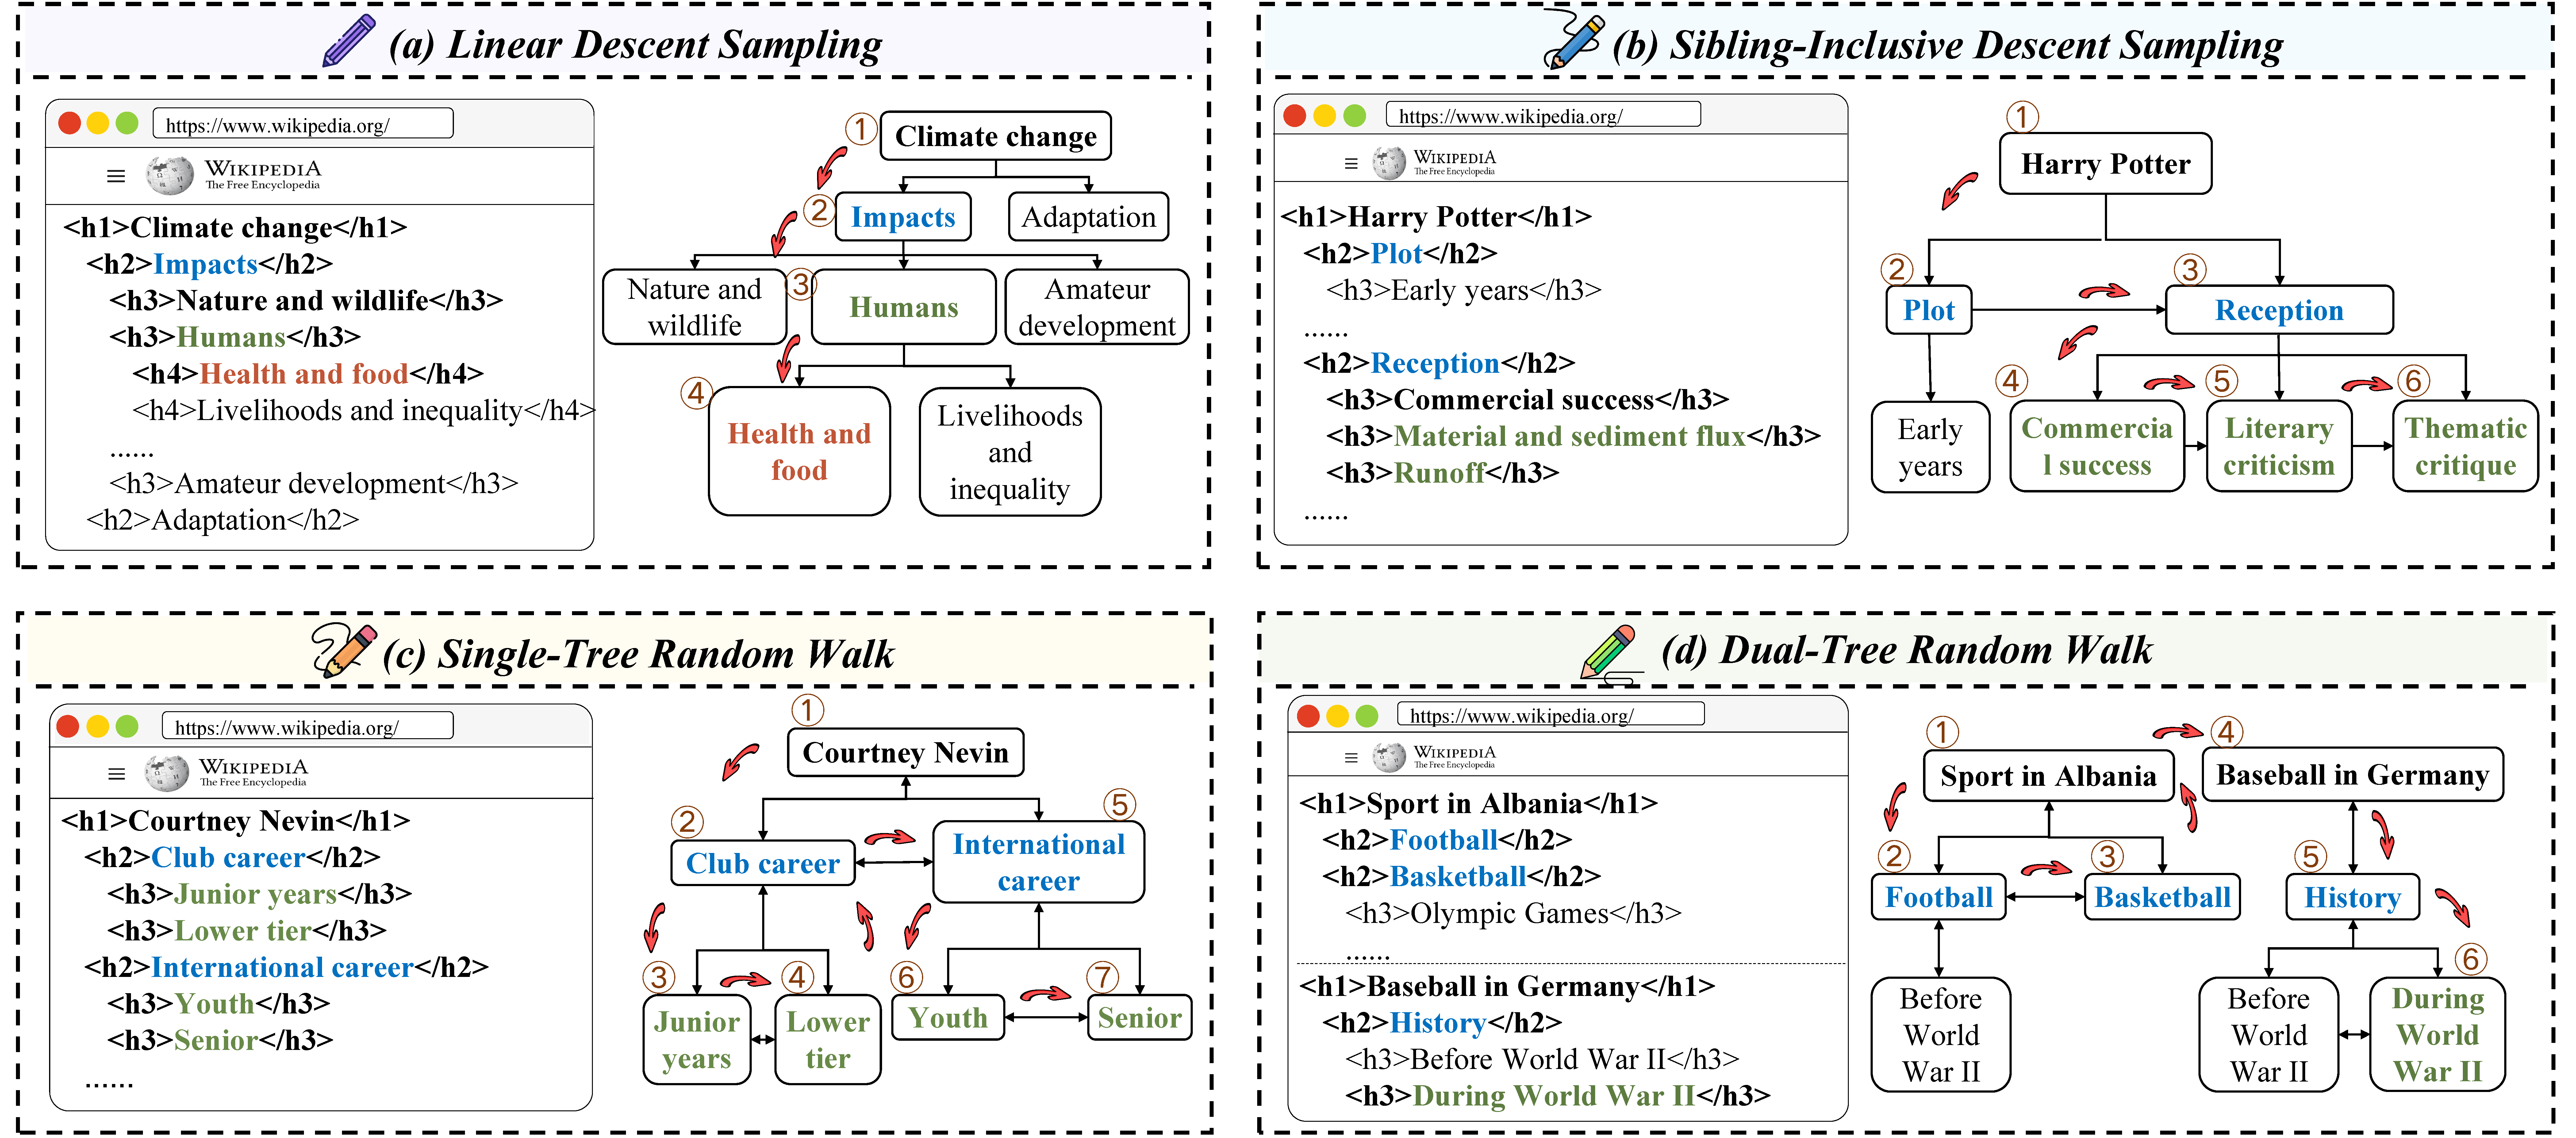
\includegraphics[width=\linewidth]{pictures/tree.pdf}
  \caption{Illustration of the four sampling strategies. The red arrows show the sampled conversation flow, with numerical labels on the nodes indicating the round of the sampled conversation turns.}
  \label{fig:title_tree}
\end{figure*}


\section{CORAL}
%In this section, we introduce our automatic approach for constructing the CORAL benchmark based on Wikipedia web pages and LLMs.

% Fundamentally, a dataset used for benchmarking conversational RAG should meet five criteria: (1) open-domain coverage, (2) knowledge-intensiveness, (3) free-form response generation, (4) handling of topic shifts, and (5) citation labeling.
% However, a comprehensive benchmark for training and evaluating these systems is lacking. 
% % The dataset must also cover a diverse range of dialogues to enhance model adaptability across different scenarios.
% We bridge this gap by proposing CORAL. This section introduces the task setup, data source, construction process, and statistics of our CORAL benchmark.



\subsection{Data Source}
\label{sec:data_source}
We choose Wikipedia as our data source for the following reasons, which align with the critical features in Table~\ref{tab:dataset_comparison}.
(1) Wikipedia pages are well-structured and enriched by global volunteers, covering a broad range of topics;
(2) The logically interconnected titles provide a strong foundation basis for generating diverse queries, with each representing a distinct intent.
(3) The human-authored content under each title includes references that not only allow for free-form responses with precise citation labeling but also serve as the golden retrieval evidence for their respective titles.


%因此，我们选择将the logically interconnected (sub-)titles 作为 an excellent basis for formulating questions, and the detailed content under each (sub-)title can serve as the corresponding free-form responses. And most claims can be supported by the citations in the References section.


However, the content may include noisy text, and reference pages are often too long for effective retrieval. 
We follow previous work~\cite{qian_webbrain} to clean the Wikipedia pages. Specifically,
for content, we remove Wikipedia templates, special symbols, and other invalid text. 
For references, we first split the reference pages into smaller passages. Then, we exclude passages shorter than 16 words or with a non-English token ratio exceeding 0.3, and then calculate term recall to identify suitable passages. After these refinements, we generate a clean set of 20,000 high-quality pages for subsequent conversations.

%To ensure the high quality and diversity of CORAL, we choose WebBrain-Raw dataset~\cite{qian_webbrain} as the data source. WebBrain-Raw originates from English Wikipedia articles, encompassing 14.86M Wiki Pages. This choice is grounded in several key factors: Firstly, the articles are carefully structured and enriched by contributions from global volunteers, ensuring extensive content coverage. Secondly, the logical interconnection of subheadings within the articles enables us to construct logically coherent conversations. Thirdly, the detailed and well-cited sections of each article can be used as responses in CORAL. Finally, the WebBrain-Raw dataset undergoes extensive refinement to eliminate noise related to content and references.

%Considering the data quality imbalance in the WebBrain-Raw dataset, we implement a filtration process to eliminate uncivil, duplicate, and incomplete entries. Following this cleansing, we conduct a random sampling of the refined dataset to ensure a representative selection.


%When constructing the CORAL dataset, we focus on five key aspects to ensure its quality:
%\textbullet\ \textit{Conversation Structure:} Ensures logical flow and natural transitions in topics, simulating real human dialogues.
%\textbullet\ \textit{Conversation Topics:} Centers on knowledge-intensive topics that require information retrieval for response generation.
%\textbullet\ \textit{Conversational Questions:} Requires references and omissions related to previous dialogue history.
%\textbullet\ \textit{Conversational Responses:} Demands precise citation labeling to confirm the source and verify the accuracy of the provided information.
%\textbullet\ \textit{Dataset Diversity:} Includes a diverse range of dialogue scenarios to evaluate the model's flexibility and effectiveness across different contexts.

%meticulously structured and enriched by contributions from global volunteers. These pages feature logically interconnected subheadings, where content under each is extensive, detailed, and well-cited. 
%This structure is perfect for use in conversational RAG dataset, where topics typically require retrieval capabilities to answer and exhibit a high degree of diversity, aligning perfectly with our dataset’s requirements for conversation topics, responses, and diversity.
%这个content可以作为我们数据集中的conversational response。并且他的topic基本上都需要检索才能进行回答，而且很diversity。完美符合我们对一个conversational rag数据集里第二点第四点和第五点的要求。
%To ensure the data quality, the WebBrain-Raw dataset undergoes extensive refinement, both in terms of article content and references.
%For the article content, WebBrain-Raw removes page templates, special symbols, and invalid elements such as images, tables, and empty sections. For the references, WebBrain-Raw carefully analyzes citations within Wikipedia to ensure that factual statements are accurately supported by relevant sources.

%\url{https://www}



\subsection{The CORAL Dataset Construction}
We transform one or more related Wikipedia web pages into information-seeking conversations through a three-stage approach.

\subsubsection{Extracting Title Trees}
First, we extract all subheadings (i.e., titles) from the raw HTML of the Wikipedia pages. These subheadings create a natural hierarchy for the content, enabling us to construct a title tree, where the page title (H1-level heading) serves as the root. Subsequent headings (e.g., H2 to H6) divide the content into progressively detailed sections, with each level corresponding to a node's depth in the tree. The directional links between nodes will dictate the flow of the generated conversations.
Besides, to enhance the complexity and diversity of conversations, we also adjust the depth, breadth, multi-subtopic exploration, and topic shifts during the construction of these title trees.

\subsubsection{Conversation Flow Sampling}\label{sec:conv_flow}
To generate coherent and diverse conversations, we implement the following four sampling strategies based on the extracted title trees:

(1) \textit{Linear Descent Sampling (LDS)}: This strategy begins at the root node and permits movement only from parent nodes to their child nodes. LDS serves as the most basic sampling path, emulating the progressive logic typical of real conversational information-seeking scenarios. As illustrated in Figure~\ref{fig:title_tree}(a), the title tree starts with the overall theme of climate change and progressively narrows down to specific impacts associated with this global issue. Following the red arrow, the focus shifts to the human aspects, particularly examining how climate change affects human health and food security. This structure exemplifies a gradual deepening of the query intent as the conversation unfolds.

(2) \textit{Sibling-Inclusive Descent Sampling (SIDS)}: This strategy builds on LDS by introducing directional links between sibling nodes. This feature is essential because conversational processes often encompass both in-depth and parallel explorations of related subtopics.
As shown in Figure~\ref{fig:title_tree}(b), when discussing the reception of Harry Potter, the subsequent three rounds of dialogue analyze it from three distinct perspectives: commercial success, literary criticism, and thematic critique. This enhancement enriches the breadth of discussions within the conversation structure.

(3) \textit{Single-Tree Random Walk (STRW)}: This strategy further enhances SIDS by incorporating interconnections among sibling nodes as well as between parent and child nodes. Essentially, it forms a directed graph with bidirectional edges. As illustrated in Figure~\ref{fig:title_tree}
(c), after an in-depth exploration of Courtney Nevin's club career, the focus shifts to her international career.

(4) \textit{Dual-Tree Random Walk (DTRW)}: It mimics the topic shifts that occur in real conversational scenarios, allowing for greater flexibility. It enables transitions between two different but somewhat related trees, which are retrieved using the root title as a query and employing the BM25 algorithm. As illustrated in Figure~\ref{fig:title_tree}(d), the conversation shifts from sports in Albania to baseball in Germany.



% By traversing the tree, we can generate a coherent dialogue.

% To construct a logically structured dialogue based on a Wiki page, we design an HTML-Tree-Conversation converting pipeline.
% We begin by mapping each subheading in the HTML to a node in the title tree. By traversing the tree, we can generate a coherent dialogue.
 %The entire tree corresponds to a complete set of dialogues. 
%we first create the title trees derived from the Wiki pages. Each node in this title tree corresponds to a subheading, representing a potential query intent.
%The content under each subheading serves as the response to that query. Additionally, the references cited in each section are treated as passages relevant to the query intent. 
%The next step involves converting each node into a complete question, which is then transformed into a conversational query to align with a natural dialogue flow.
% 树上的一个节点对应一个turn，一棵树对应一组对话



% \subsubsection{HTML-Tree Stage}
% % 由于wikipedia page中，有多级标题来组织这个页面形式，因此各级标题之间有逻辑关系
% In HTML, subheadings establish a logical hierarchy for content. We utilize this structure to extract subheadings and create a title tree, where the page title (H1-level heading) acts as the root. Subsequent headings, from H2 to H6, divide the content into progressively detailed sections. Each heading level directly corresponds to a node's depth in the title tree, creating a hierarchical structure that reflects the organization of the article. The directional links between nodes decide the flow of conversation generated in the later stage.

% Therefore, we choose to design diverse directional links between nodes to simulate the logical relationships between dialogue turns in real conversational scenarios. Based on the directional links, the title tree can be categorized into four distinct types shown in Figure~\ref{fig:title_tree}. Specific details are as follows:


%\noindent \textbf{Hierarchical Relationships}: General to specific, like a "Climate Change" page with "Impacts" and "Extreme Weather Events."
%Decompositional: Breaking down complex topics, such as "Renewable Energy" with "Solar Energy" and "Wind Energy."
%Chronological: Arranging by time, like a "History of Computing" page with "Early Computers" and "Modern Computing."
%Geographical: Sorting by regions, exemplified by "World Languages" with "European Languages."
%Causal: Showing cause and effect, such as a "Public Health" page with "Causes of Obesity" and "Preventive Measures."
% \begin{itemize}
%     \item \textit{Parent-Child Tree.} 
%\noindent \textbf{Parent-Child Tree(PCT).} 
% We design the Parent-Child Tree (PCT), the most fundamental tree structure crafted to emulate the typical progressive logic observed in real conversational scenarios. The PCT is organized hierarchically in a top-down manner, where each directed edge points from the parent node to its child nodes. As illustrated in Figure~\ref{fig:title_tree}(a), the title tree starts with the overarching theme of climate change and progressively delves into specific impacts associated with this global issue. Following the red arrow, the focus narrows down to the human aspects, particularly examining how climate change affects human health and food security. This structure represents a progressive deepening of the query intent as the conversation unfolds.

% \item \textit{Parent-Sibling Tree.}
% The Parent-Sibling Tree (PST) expands on the PCT by introducing directional links between sibling nodes. This feature is essential as it is widely recognized that in conversational processes, the evolution of query intents encompasses not only deeper explorations but also parallel comparisons among related subtopics. As shown in Figure~\ref{fig:title_tree}(b), when discussing the reception of Harry Potter, the subsequent three rounds of dialogue deconstruct it from three distinct perspectives: commercial success, literary criticism, and thematic critique. This enhancement enriches the breadth of discussions within the tree structure. 

% \item \textit{Parent-Sibling-Child Interconnect Tree.}
% Considering the necessity of exploring multiple subtopics within a single topic, we propose Parent-Sibling-Child Interconnect Tree(PSCT). The PSCT further enhances the PST by incorporating interconnections not only among siblings but also between parents and children. Essentially, it forms a directed graph with bidirectional edges. As illustrated in the Figure~\ref{fig:title_tree} (c), following an in-depth exploration of Courtney Nevin's club career, the focus will shift to her international career.


% \item \textit{Dual Parent-Sibling-Child Interconnect Trees.}
% To mimic the topic shifts that occur in real conversational scenarios, we design the Dual Parent-Sibling-Child Interconnect Trees (DPSCT). We combine two PSCTs into a unified structure. First, we prompt LLM to generate topics associated with the first tree. Then, we use these generated topics to retrieve the root of the second tree, identifying potential logical connections between the two PSCTs. As illustrated in Figure~\ref{fig:title_tree} (d), the topic shifts from sports in Albania to the baseball in Germany.
% \end{itemize}





\subsubsection{Contextualization of Questions}
\label{question_generation}
As introduced in Section~\ref{sec:data_source}, we treat the subtitles as the sources of questions, with their corresponding contents serving as the responses. In this final stage, we contextualize the keyword subtitles into conversational questions to enhance the realism of the conversation.

Specifically, for each turn, we first create a keyword chain that includes the current node and all its ancestor nodes. This keyword chain, along with the response of the current node, is then used to prompt GPT-4\footnote{gpt-4-turbo-2024-04-09 from https://openai.com/api\label{gpt-4}} to rewrite the original keyword title into a natural language question. We then continue to prompt GPT-4 to further contextualize the question into a conversational format by incorporating linguistic phenomena such as ellipses, references, and omissions~\citep{cast19}, which are prevalent in real conversational scenarios.
The prompt details are provided in Appendix~\ref{prompts_of_contextualization_of_questions}.

% Secondly, considering the linguistic phenomena such as ellipses, references, and omissions~\citep{cast19} prevalent in real conversational scenarios, we prompt LLM\textsuperscript{\ref{gpt-4}} to transform the complete question into the conversational question. The complete prompt with an example is shown in Table~\ref{prompt_of_generating_conversational_question}

% \subsubsection{Tree-Conversation Stage}
% \label{question_generation}
% As shown in Figure~\ref{fig:overview} (a), by traversing the title tree, we can create a coherent conversation. Converting tree nodes into conversations consists of two steps.


% Firstly, we convert the tree node into the complete question. Each subheading in the title tree represents a potential query intent, with the content beneath each heading serving as the corresponding response. References cited in each section are treated as passages relevant to the purpose of the query.
% % 介绍keyword chain
% To generate a complete question, we construct a keyword chain that includes the current node and all its ancestor nodes. The keyword chain, together with the response for the current node, is then used to prompt LLM\footnote{gpt-4-turbo-2024-04-09 from https://openai.com/api\label{gpt-4}} to reconstruct the original question. The complete prompt with an example is shown in Table~\ref{prompt_of_generating_question}.

% Secondly, considering the linguistic phenomena such as ellipses, references, and omissions~\citep{cast19} prevalent in real conversational scenarios, we prompt LLM\textsuperscript{\ref{gpt-4}} to transform the complete question into the conversational question. The complete prompt with an example is shown in Table~\ref{prompt_of_generating_conversational_question}. %\footnote{We put Table~\ref{prompt_of_generating_question} and Table~\ref{prompt_of_generating_conversational_question} in Appendix~\ref{sec:appendix} due to the space limitation. See our open-sourced code for the full prompt.}

%While in most human conversations, elements such as ellipsis, references, and omissions~\citep{cast19} are common, where pronouns and implied contexts allow for the omission of words that can be inferred from previous exchanges. Our conversational questions are designed to mimic human conversations, ensuring smooth and coherent transitions between turns. By incorporating typical conversational phenomena such as coreferences and omissions, we aim to enhance the natural flow of the dialogue. Inspired by the power of the LLMs, we prompt the LLM to use chain-of-thought~\citep{wei_nips22_cot} to transform the question into the conversational question. The complete prompt with an example is shown in Table~\ref{prompt_of_generating_conversational_question}.

% Ultimately, we develop the CORAL dataset that features logical relationships between turns and includes citation labeling in the responses.


\begin{table*}[htbp]
    \centering
    \setlength{\tabcolsep}{12pt}
    \small % 如果0不行，尝试+1或-1来找到合适的大小
    \begin{tabular}{@{}ccccccc@{}}
        \toprule
        Category & Method & MRR & MAP & NDCG@3 & Recall@20 & Recall@100 \\
        \midrule
        
        \multirow{4}{*}{CDR Models} &Conv-ANCE-Q & 19.8 & 28.6 & 20.5 & 39.1 & 51.0 \\
        &KD-ANCE-Q & 22.6 & 33.1 & 24.5 & 38.5 & 48.0 \\
        &Conv-ANCE-C & 20.5 & 29.6 & 21.1 & 39.8 & 53.4 \\
        &KD-ANCE-C & \textbf{23.2} & \textbf{33.6} & 24.9 & \textbf{40.3} &\textbf{49.6} \\
        
        \midrule
        \multirow{3}{*}{CQR Models} &LLM4CS (GPT-3.5) & 21.2 & 31.1 & 23.0 & 35.5 &44.4 \\
        &Qwen2.5-1.5B & 16.3 & 23.8 & 17.2 & 31.0 & 39.2 \\
        &Qwen2.5-1.5B-SFT & 23.1 & \textbf{33.6} & \textbf{25.1} & 39.4 &48.6 \\
        %\midrule
        %&Original Question  & 23.6 & 34.2 & 25.5 & 40.1 & 49.0 \\
        \bottomrule
    \end{tabular}
    \caption{Retrieval performance comparisons. The best performance is \textbf{bold}.
    %\textit{Original Question} denotes using the generated question based on the keywords as introduced in the section~\ref{question_generation}. 
    \textit{Conv-ANCE-Q} denotes the Conv-ANCE is trained on the QReCC dataset and \textit{Conv-ANCE-C} denotes the Conv-ANCE is trained on CORAL training dataset.}
    \label{conversational_search_performances}
\end{table*}


\subsection{The Final Dataset Format and Statistics}
The key statistics of CORAL are summarized in Table~\ref{statistics_four_conversation_structures}. Our dataset consists of 8,000 conversations with the four types introduced in Section~\ref{sec:conv_flow}. These 8,000 conversations are evenly distributed across four distinct structural types, with each type containing 2,000 conversations. Specifically, the LDS conversation type includes 3 to 6 turns per conversation. For the remaining types—SIDS, STRW, and DTRW—each category consists of 1,600 sets of conversations with 6 to 10 turns, along with an additional 400 sets featuring 11 to 20 turns per conversation. The design of the longer conversation intends to simulate real-world challenges encountered in conversational scenarios, such as redundant information and the long context problem. 

Our final dataset format is as follows: A conversation $\mathbf{C}=\{ (q_{i},r_{i})\}_{i=1}^{n}$ comprised of $n$ turns. $q_{i}$ is a contextualized query of the $i$-th turn generated in Section~\ref{question_generation}, and $r_{i}$ is the $i$-th turn golden response, which is the cleaned plain text under the corresponding (sub-)title in the HTML.
%(introduce what the response is).
The supporting web pages for $r_{i}$, listed in the HTML Reference Section, can be processed as described in Section~\ref{sec:data_source} to serve as the golden relevant passages $P_i^+ = \left\{ p_{i,1}, p_{i,2}, \ldots \right\}$.
%$r_{i}$ has supporting web pages in the Reference Section, after cleaning, can serves as the corresponding golden relevant passages $P_i^+ = \{ p_{i,1},p_{i,2},...\} $.
%$r_{i}$ has the associated supporting references $P_i^+ = \{ p_{i,1},p_{i,2},...\} $, which serves as the corresponding golden relevant passages.
%These references are related web pages listed in the HTML Reference Section.
%(citations)...introduce the citation label related data here. give symbols and these symbols should be consistent with Section 3.3.
On average, each conversation turn has 3.17 related passages, and the average golden response length is 255 tokens. Finally, we obtain a passage corpus $\mathcal{P} $, which contains 200K passages from all the golden references $P_i^+$.


%Introduce the retrieval passage corpus $\mathcal{P} $  in 1-2 sentences, back linking to 3.1. give the number of passages in the corpus.




\subsection{Evaluation Tasks}
CORAL mainly supports three fundamental conversational RAG tasks:

(1) \textit{Conversational Passage Retrieval}:
This task evaluates a system's capability to extract relevant information from extensive document collections, considering the context of multi-turn conversations. Formally, given the $k$-th question $q_{k}$ and the corresponding conversation history
% $ H_{k} =\left \{ q_{1},r_
% {1},q_{2},r_{2}...,q_{k-1},r_{k-1}\right \} $
$H_{k} = \{ q_{i},r_{i}\}_{i=1}^{k-1}$, where $q
_{i}$ and $r_{i}$ respectively denote the question and response of the $i$-th turn, the retriever $\mathbb{R} $ aims to retrieve the relevant passages
$P_{k} $
from the passage corpus $\mathcal{P} $. 
%Following previous conversational search work~\cite{mele_sigir20,mao_emnlp22_convtrans,mo_acl23_cqr,CONVINV_cheng_acl24}, 
We use
MRR, MAP, NDCG@3, Recall@20 and
Recall@100 as retrieval evaluation metrics.



(2) \textit{Response Generation}: This task challenges the system's ability to produce accurate, detailed, and contextually appropriate answers.
Given the $k$-th question $q_{k}$, the corresponding conversation history $ H_{k} $, and the relevant passages  $P_{k}$, the generator $\mathbb{G} $ needs to generate an informative response to answer the question. We use rule-based metrics BLEU-1~\cite{bleu}, and ROUGE-L~\cite{lin2004rouge} to evaluate the response quality compared with $r_{k}$. Given the lengthier responses in our benchmark, we additionally utilize the model-based evaluation method proposed in RichRAG~\citep{wang_richrag}.



(3) \textit{Citation Labeling}: This task evaluates the method's ability to accurately attribute information sources within the generated responses.
Following ALCE~\citep{gao_alce_emnlp23}, the generated response $r_{k}$ consists of $n$ statements $s_1, s_2,...,s_n$. Each statement $s_i$ cites a list of passages $C_i = \{ c_{i,1},c_{i,2},...\} $, where $c_{i,j} \in P_k$. We adopt Citation Recall and Citation Precision defined in ALCE~\citep{gao_alce_emnlp23} to evaluate the accuracy of citation labeling.

%------the first version------

%Given the $k$-th question $q_{k}$, the corresponding conversation history $ H_{k} $, and the relevant passages  $p_{k}^{+}$. The generator $\mathbb{G} $ needs to generate a response $r_{k}$ with citation labeling. For example, if the retrieved passage with passage ID 2 and 5 respectively support the first and the second generated sentences in the response, the output should follow the format: ``$sent_{1} ^{\left [2\right ]}. sent_2 ^{\left [5\right ] }...$''.

%--the second version---







\begin{table*}[tbp]
    \centering
    \setlength{\tabcolsep}{11pt}\renewcommand{\arraystretch}{0.9}
    \setlength{\tabcolsep}{4pt}
    \small % 如果0不行，尝试+1或-1来找到合适的大小
    \begin{tabular}{@{}p{2.8cm}p{1.5cm}lcccc@{}}
        \toprule
        \multirow{2}{*}{Category} & \multirow{2}{*}{\textbf{\# Tokens}} &\multirow{2}{*}{Model} & \multicolumn{2}{c}{Generation} & \multicolumn{2}{c}{Citation Labeling} \\
        \cmidrule(lr){4-5}
        \cmidrule(lr){6-7}
        & & &BLEU-1 & ROUGE-L & Citation Recall & Citation Precision \\
        \midrule

        \multirow{6}{2.8cm}{Raw Context} & \multirow{6}{*}{2226} &Qwen2.5-7B &  22.2  & 13.1&3.1&18.1 \\
        &&Mistral-7B & 18.1 & 12.4 &2.4 &4.8\\
        &&Llama-3.1-8B & 21.5 & 12.9 & 0.9 & 2.1\\
        \cmidrule(lr){3-7}
        &&Qwen2.5-7B-SFT & 18.3 &  18.5 & 6.6& 16.8\\  
        &&Mistral-7B-SFT & 23.7  & \textbf{20.1} & 4.6 & 11.1\\
        &&Llama-3.1-8B-SFT & 24.2 & 19.7 & 4.2 & 9.8\\

        \midrule
        
        \multirow{6}{*}{Last Response} &\multirow{6}{*}{1474} &Qwen2.5-7B & 20.9 & 12.8 & 3.5 & 20.8 \\
        &&Mistral-7B & 18.1  & 12.3 & 2.7 & 4.5\\
        &&Llama-3.1-8B & 20.4 & 12.7 & 1.3 & 3.1 \\
        \cmidrule(lr){3-7}
        &&Qwen2.5-7B-SFT & 23.9  & 16.5 & 10.4 & 24.8\\  
        &&Mistral-7B-SFT & 21.8 & 18.5 & 5.0 & 12.4\\
        &&Llama-3.1-8B-SFT & 26.1 & 18.1 & 3.5 & 8.7\\
        
        
        \midrule
        \multirow{6}{*}{Rewrite} &\multirow{6}{*}{1236} 
        &Qwen2.5-7B & 21.1  & 12.8 & 2.4& 9.4 \\
        &&Mistral-7B & 18.8  & 12.3 & 2.5 & 3.8 \\
        &&Llama-3.1-8B & 18.8 & 12.4 & 1.7 & 3.1 \\
        \cmidrule(lr){3-7}
        &&Qwen2.5-7B-SFT & 18.9 & 16.4 & 7.4 & 16.8\\
        &&Mistral-7B-SFT & 24.8 & 18.5 & 5.9 & 14.8\\
        &&Llama-3.1-8B-SFT & \textbf{26.3} & 18.2 & 4.7 & 11.2\\

        \midrule
        \multirow{6}{4cm}{LLM Summarization} & \multirow{6}{*}{478} 
        &Qwen2.5-7B & 21.0 & 12.7 & 2.9 & 13.0 \\
        &&Mistral-7B & 19.5 & 12.3 & 5.6 & 6.7 \\
        &&Llama-3.1-8B & 19.1 & 12.8 & 4.1 & 7.1 \\

        
        \cmidrule(lr){3-7}
        &&Qwen2.5-7B-SFT & 23.5&16.8& \textbf{14.1} & \textbf{31.1}\\
        &&Mistral-7B-SFT & 16.9 & 17.1 & 8.3 & 19.8 \\
        &&Llama-3.1-8B-SFT & 18.7 & 16.5  & 4.5 & 10.7 \\
        
        \bottomrule
    \end{tabular}
    \caption{The comparison of different LLMs on response generation and citation labeling. \textit{\# Tokens} denotes the number of input tokens. }
    \label{generation_performances}
\end{table*}





















% \section{Strategies}
% In this section, we introduce three common compression strategies of conversational RAG. 

\section{Conversational RAG Framework}
\label{sec:conversation_compression}
A conversational RAG system typically comprises a retriever and a generator to handle the current user query $q_k$, the conversation history $H_k$, and the retrieved passages $P_k$. As the conversation progresses, both the growing conversation history and the noisy retrieved passages can negatively impact the system's efficiency and effectiveness, making it harder to generate accurate responses. To solve the problem, we propose a simple compression framework to efficiently manage these inputs.
Specifically, we introduce a conversation compression function $f$ to compress the conversation, and then use the compressed contents as the real inputs of retrievers and LLM generators. In addition to conversation compression, we also apply post-retrieval results compression. Following existing approaches~\cite{xu_recomp}, we simply take LLMs as the compression function $f_{p}$, leaving the exploration of more compression methods in future work.

Formally, suppose $f(H_k)$ is the compressed conversation context, $P_k=\mathbb{R} (f(H_k), q_k)$ is list of passages retrieved by querying $f(H_k)$ with $q_k$, and $f_{p}(P_k)$ is the compressed results of the retrieval,
the final generation task can be formulated as:
$\mathbb{G}(q_k, f(H_k), f_{p}(P_k)) $. The prompt for feeding $q_k, f(H_k), f_{p}(P_k)$ into the generator can be found in Appendix~\ref{prompts_of_generating_responses}.
%
Various existing conversational RAG methods can be unified into our framework. In this work, we mainly investigate the following three methods for the conversation compression:

\paragraph{Last Response Strategy} 
For the conversation history, 
we heuristically select all previous conversational questions $\{q_{i}\}_{1}^{k-1}$ and the last turn's response $r_{k-1} $ in the conversation history:
\begin{eqnarray}
    f^{\text{LR}}(H_k)=\{q_{i}\}_{1}^{k-1},r_{k-1}.
\end{eqnarray}
%We then feed $f^{\text{LR}}(H_k)$ along with the current question $ q_{k} $, and retrieved passages $p_{k}^{+}$ into the LLM generator $\mathbb{G} $ to generate cited responses $r_k$. %This process is represented as $r_{k} = \mathbb{G}  \left ( q_k;H'_k;p_{k}^{+} \right )  $.

\paragraph{Rewrite Strategy}
We adopt a conversational query rewriting model Rewrite() to transform the original query along with the conversation history into a standalone question
rewrite $\hat{q_k}$:
\begin{eqnarray}
    f_{c}^{\text{RW}}(H_k) =\hat{q_k} = \text{Rewrite}\left(q_k;H_k \right).    
\end{eqnarray}
In this strategy, $P_k=\mathbb{R} (\hat{q_k})$ is list of passages retrieved by querying $\hat{q_k}$, and $f_{p}(P_k)$ is the compressed results of the retrieval,
the final generation task can be formulated as:
$\mathbb{G}(\hat{q_k}, f_{p}(P_k)) $.

\paragraph{LLM Summarization Strategy}
Inspired by RECOMP~\citep{xu_recomp}, we use LLMs to generate abstractive summary of the conversation history:
\begin{eqnarray}
    f_{c}^{\text{SUM}}(H_k) = \text{LLM}(H_{k}).
\end{eqnarray}
The prompt is shown in Appendix~\ref{prompts_of_LLM_summarization_strategy}.



% a  compress the conversation and the retrieved passages simu
% . These summaries, along with the current question $q_k$, are then input into the generator $\mathbb{G}$ to produce the cited response $r_k$. This can be expressed as $r_k = \mathbb{G}(q_k; H_k^s; p_k^s)$.
% skimmed milk

% skimmed milk
%  对话历史建模与skim passages
% 考虑到冗长的对话历史可能会给大模型理解用户查询意图带来困扰，因为对话历史中经常存在一些topic shift或者存在回答太长的问题，会干扰大模型。
% 所以我们选择对对话历史进行summarize，重新建模对话历史，让他变得易于被llm理解之前用户的查询意图与接收到的信息
% 与此同时，inspred by recomp那篇工作，我们还选择对检索得到的passage进行summarize，这样不仅可以..还可以...
% 我们使用了一个abstractive compressor来对检索得到的文档进行提炼，保证提炼后的文档确实存在相关信息能用来帮助回答问题。




\section{Experiments}


In this section, we discuss the performance of conversational RAG on our benchmark, and provide a comprehensive analysis for each stage.



%\subsection{Main Results}
\subsection{Evaluating Retrieval Performance}

%Q删掉
%DGT comment，分析思路：
%1；Existing convRAG baselines show valunable performance in Coral，并且较好的baseline仔五个指标上。
%2: category CDR 与 CQR show 相似性能表现，值得注意的是 Qwen 2.5 1.5B sft不仅强于Qwen instruct Version，甚至有强于powerful close source LLM的性能
% 3. KD-ANCE > Conv-ANC， 方法设计的角度去想想，可能的原因是xxx
We concentrate on two main approaches in conversational search: conversational dense retrieval (CDR) and conversational query rewriting (CQR). For CDR, we use KD-ANCE and Conv-ANCE with ANCE as the base retriever. KD-ANCE~\citep{yu_sigir21_cdr} trains the session encoder by mimicking golden query embeddings, while Conv-ANCE~\citep{Karpukhin_dpr_emnlp20,lin_emnlp21_cdr} uses contrastive learning to train the session encoder, drawing it closer to relevant passages and further from irrelevant ones. For CQR, we utilize the LLM4CS~\citep{mao_emnlp23_llm4cs}, which incorporates GPT-3.5, and an open-source LLM for generating query rewrites respectively to enable a comparative analysis. Table~\ref{conversational_search_performances} provides a detailed comparison between these two categories. We have the following observations:
%(1) CDR模型中，KD-ANCE-C, exhibit superior performance in most metrics, with notable leadership in MAP (33.6) and R@100 (49.6).

\begin{figure*}[!t]
  \centering
  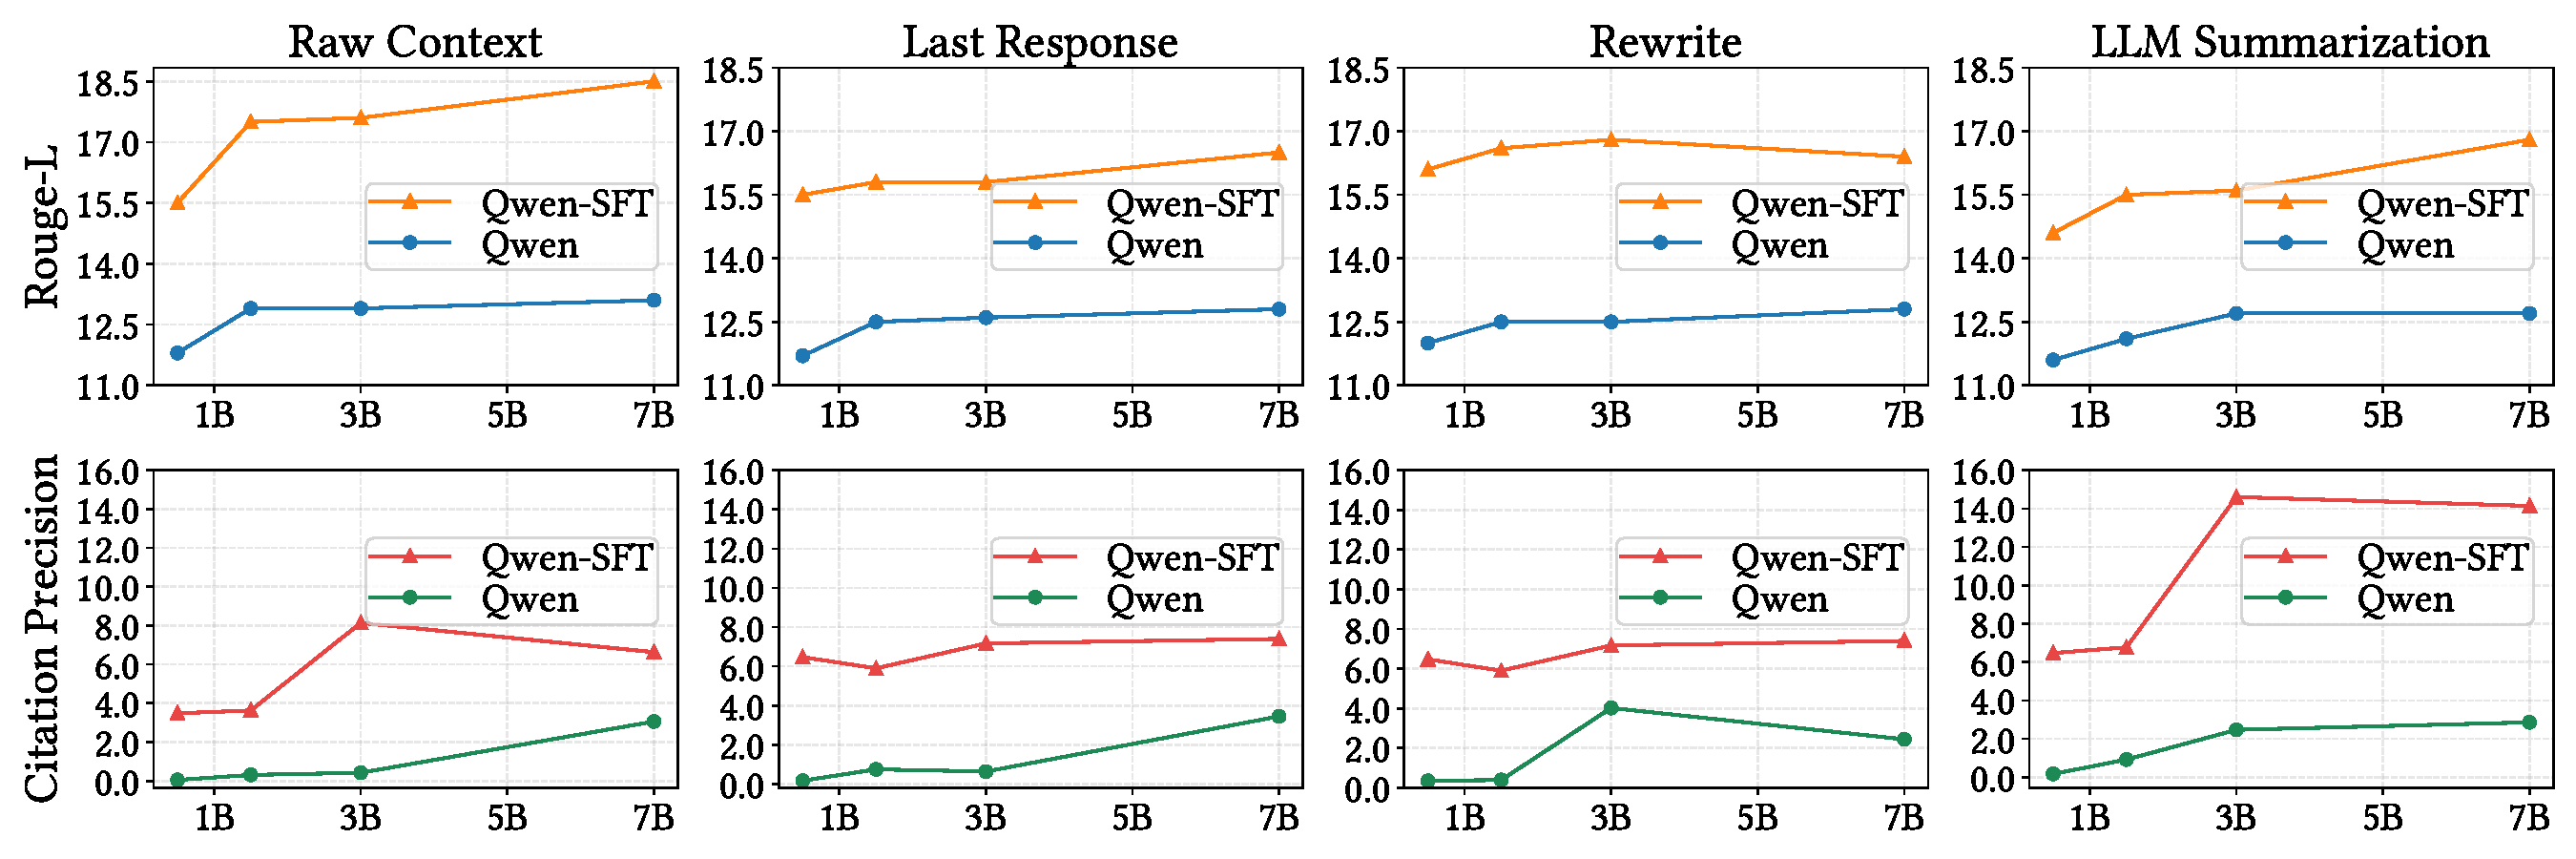
\includegraphics[width=\linewidth]{pictures/scaling.pdf}
  \caption{The scaling analysis of generation and citation labeling performance.}
  \label{fig:scaling}
\end{figure*}


\begin{figure*}[!t]
  \centering
  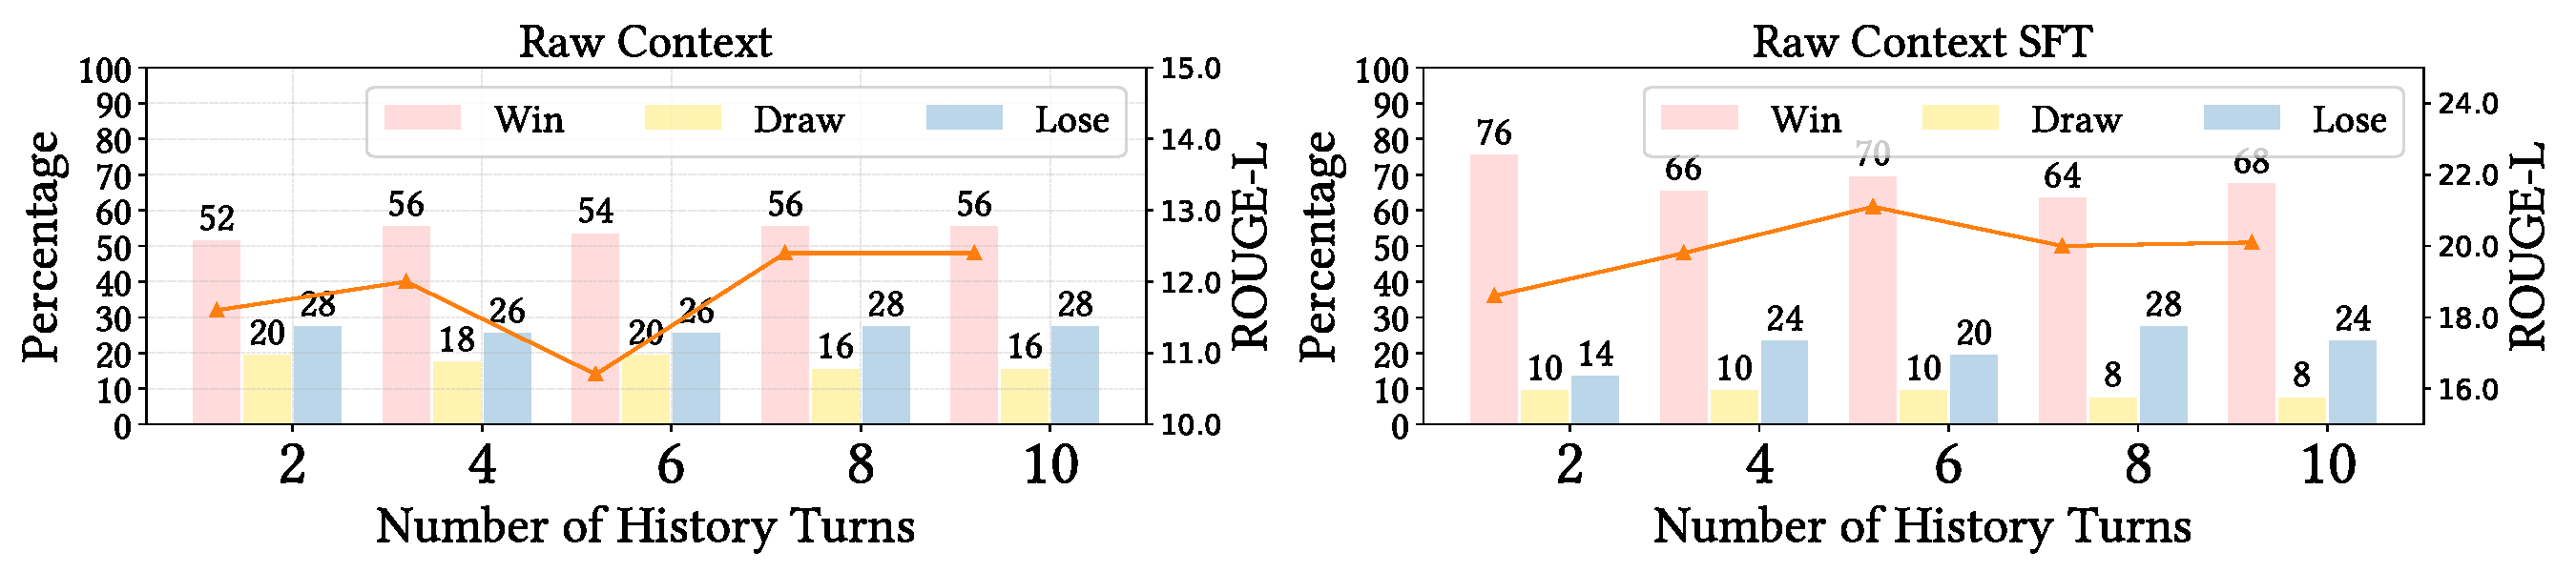
\includegraphics[width=\linewidth]{pictures/conversation_turns.pdf}
  \caption{Generation results of different conversation history length. The curve in the figure represents the ROUGE-L score. The histogram shows the results of GPT-4 scores comparing model-generated responses with golden responses. \textit{Win} indicates cases where model-generated responses outperform golden responses, \textit{Draw} indicates cases where the two responses are considered equally good, and \textit{Lose} indicates cases where the golden responses are considered better. The y-axis on the left represents the proportion of cases in the total number of cases.}
  \label{fig:irrelevant_conversation_information}
\end{figure*}


%(1) The KD-ANCE-C model within the CDR category demonstrates superior overall performance, particularly excelling in the R@20 and R@100 metrics with the highest recorded values of 40.3 and 49.6 respectively. This suggests its robustness in retrieving relevant results from longer candidate lists. In contrast, the Qwen2.5-1.5B-SFT model in the CQR category, while competitive in MAP and NDCG@3 (even slightly surpassing KD-ANCE-C in NDCG@3), falls short in performance for longer list retrievals.
%This might indicate that the model is more appropriate for applications requiring high precision rather than those needing to retrieve information from a large pool of candidates.
\begin{figure}[h]
  \centering
  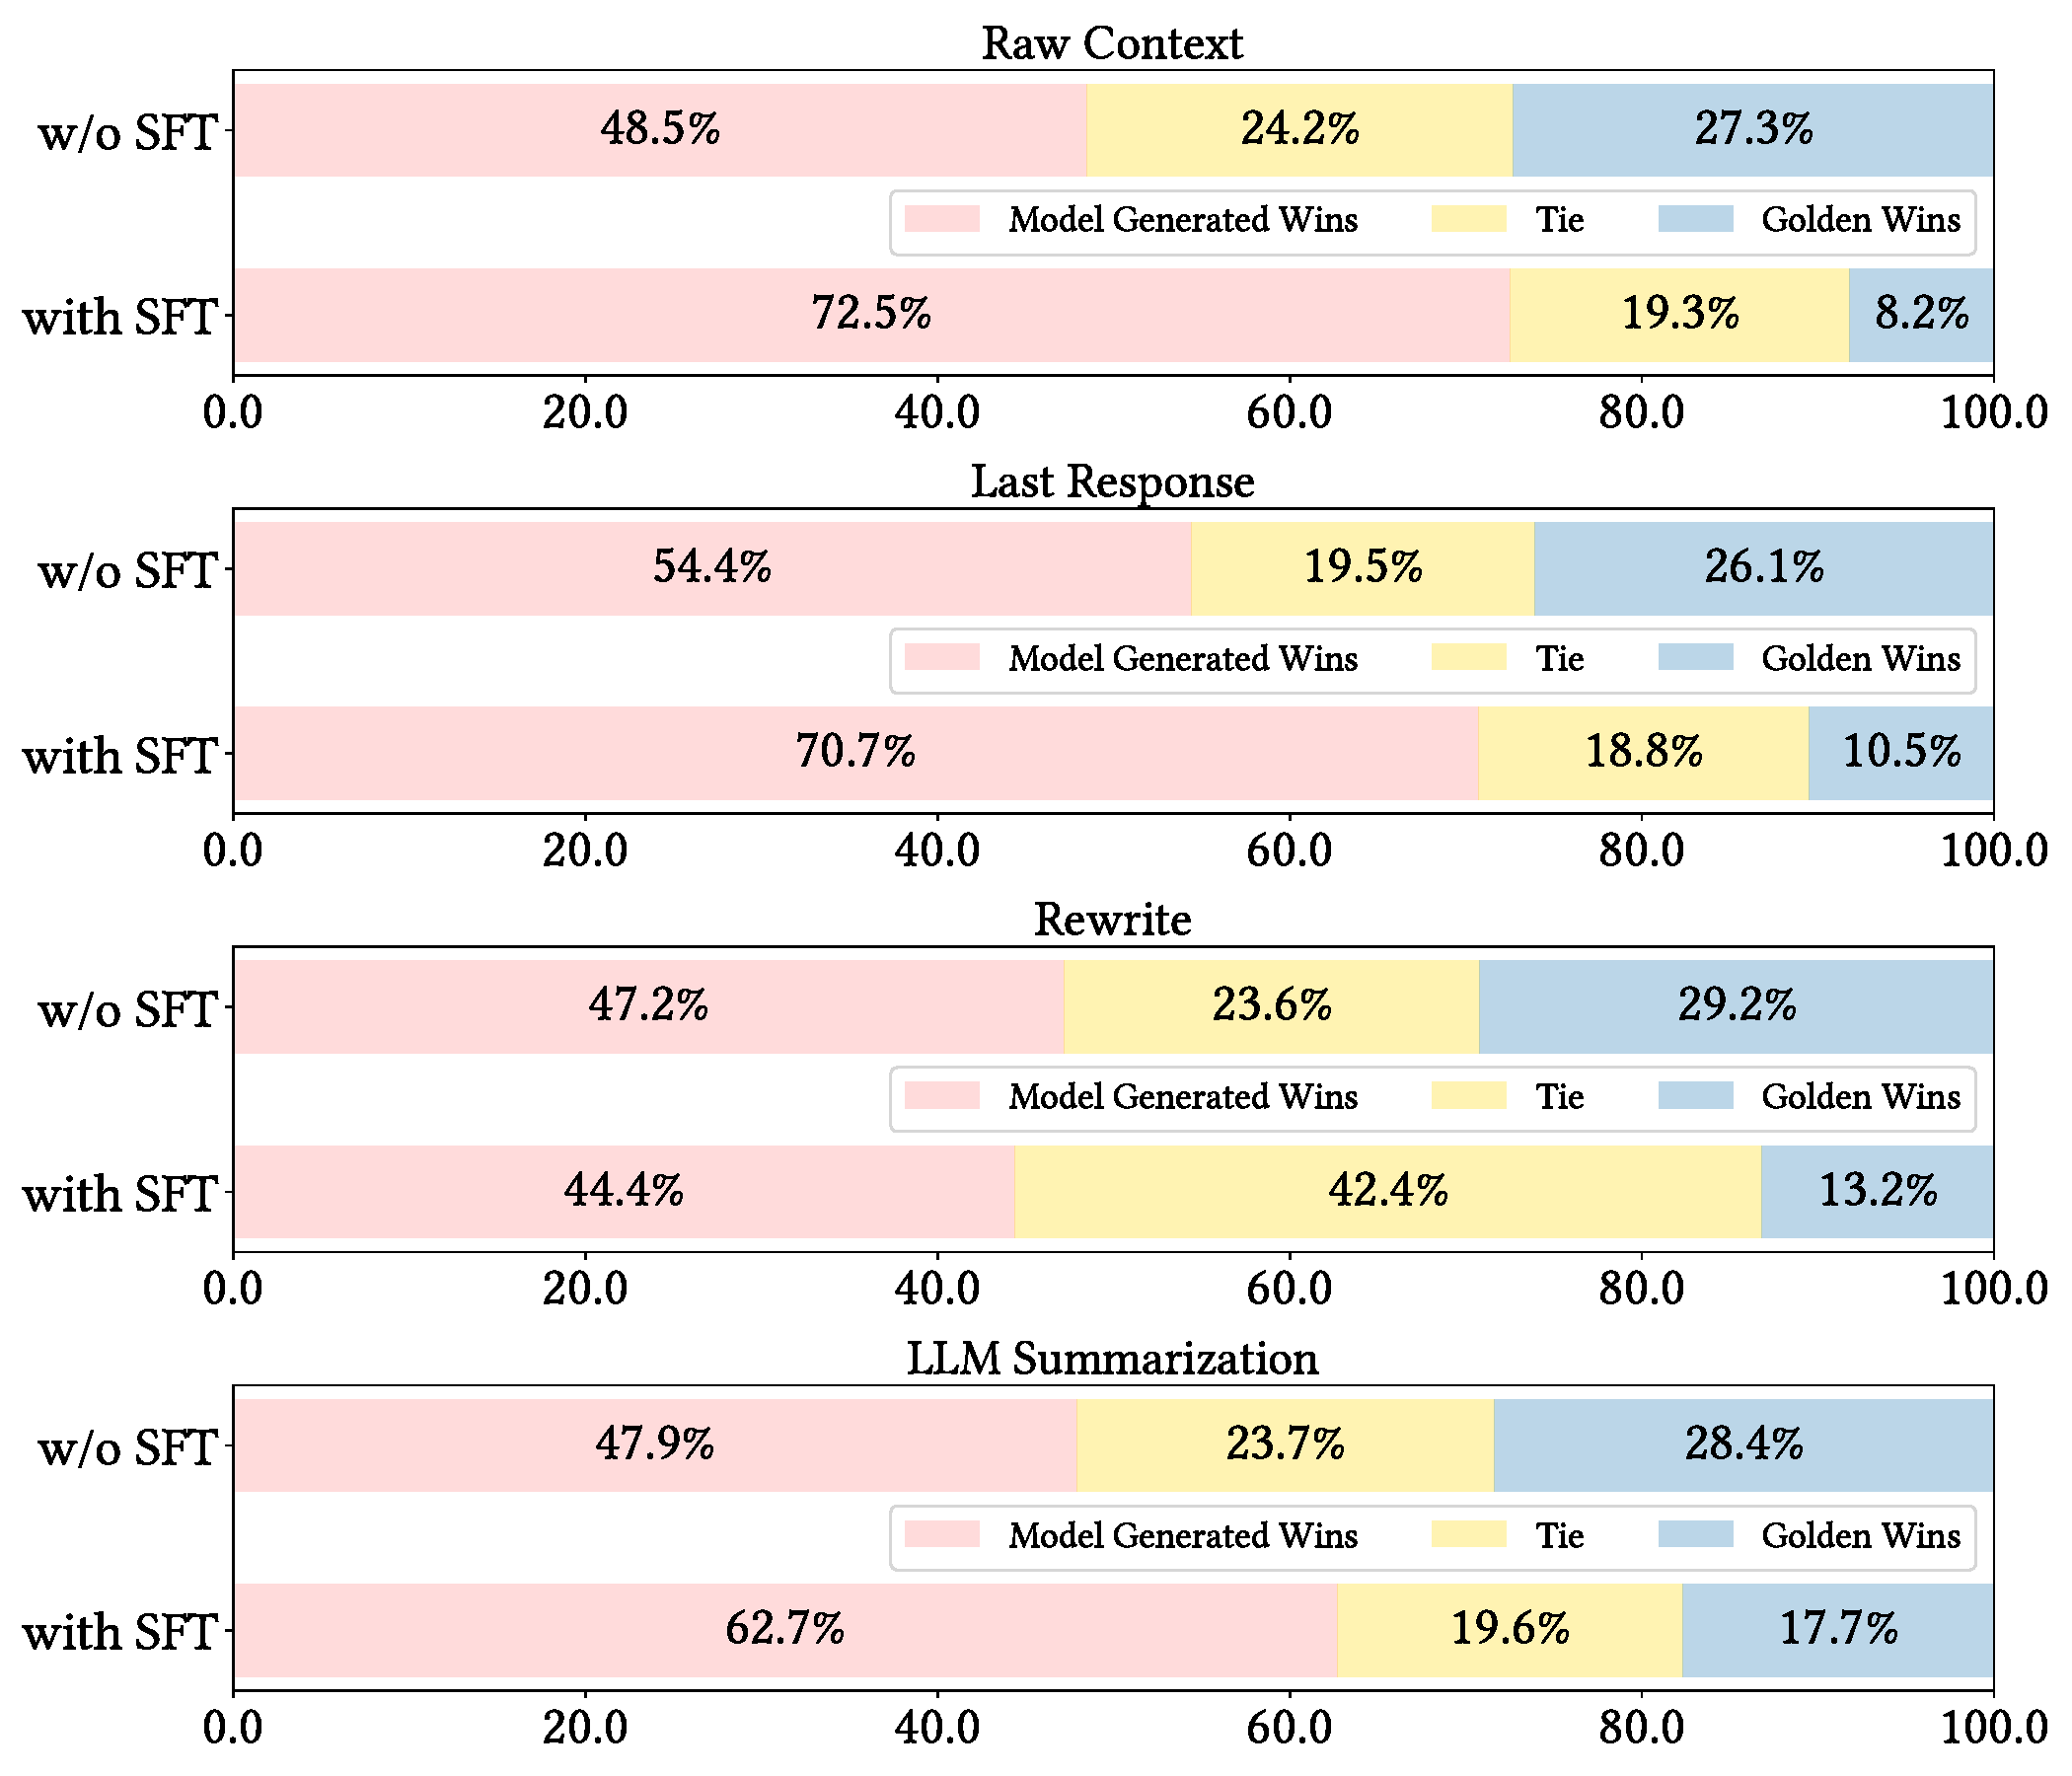
\includegraphics[width=\linewidth]{pictures/gpt_evaluation.pdf}
  \caption{The GPT-4 evaluation score.}
  \label{fig:gpt_evaluation}
\end{figure}

(1) The performances of the CDR and CQR models are fairly comparable. Notably, the Qwen2.5-1.5B-SFT shows a strong competitive edge, not only surpasses the Qwen2.5-1.5B but also outperforms the advanced closed-source LLM GPT-3.5 across all evaluated metrics.% showing improvements with increases of 1.9 in MRR, 2.1 in NDCG@3, and 4.2 in Recall@100.

(2) KD-ANCE in the CDR category shows better results compared to Conv-ANCE. This may be attributed to the training methodologies: KD-ANCE possibly leverages golden rewrite data more effectively than Conv-ANCE, which uses in-batch negatives that may not be sufficiently challenging for optimal learning.

%(3) 经过微调后的Qwen2.5-1.5B-instruct-SFT比闭源的商业大模型gpt3.5表现很好，这证明了xxxxx



%\textbf{Generation Perspective}
%DGT comment，分析思路：
% 1. 在generation维度，我们评测了3 top open sourced LLM，并结合常用的RAG结合策略，我们惊喜地发现他们在三个metric（xxx）表现出一致性的不佳（<25%）甚至在，Mentor与Rouge <15% ，可能的原因是现有top LLM在面对不相关信息及建模长窗口输入表现不佳（discussion做了细致的探讨），这也印证了我们benchmark在ConvRAG意义

%2. SFT带来的了stable的perfomance gain，无论generation or citation lableing：具体给指标

%3. 对比三个策略 Rewrite with SFT 最佳，可能的原因是xxxx，而意外的是，summarize虽然在generation表现不佳，但是结合citation labeling却又显著提升，可能的原因是：xxxx


\subsection{Evaluation Response Generation with Citation Labeling}
We compare the raw context baselines with another three conversation compression strategies introduced in Section~\ref{sec:conversation_compression}, selecting Qwen2.5, Mistral, and Llama as generators. We prompt the generator to generate the response along with the citations in the response.
The generation and citation labeling performance is shown in Table~\ref{generation_performances}, and the GPT-4 score is shown in Figure~\ref{fig:gpt_evaluation}. We find that:

(1) By examining four methods of modeling conversation history, we observe an interesting trend: as the input is progressively condensed (from 2226 input tokens in the raw context to merely 478 input tokens in the LLM Summarization), 
%there is a notable reduction in the number of input tokens. However, 
the decrease in performance is surprisingly minimal, and in terms of citation labeling, there is even an observed improvement. This suggests that some content within the dialogue history is irrelevant or redundant and can be removed without negatively impacting the model's performance.

%(2) Compared to models without fine-tuning, the SFT model exhibits better performance in both response generation and citation labeling, particularly noticeable with at least 3.6 increase in the ROUGE-L metric.
%Rewrite-Qwen-2.5-7B


(2) Among three conversation compression strategies, the Rewrite with SFT exhibits superior performance, which could be attributed to the model's enhanced capability to learn from the simplified question-answer pattern. Intriguingly, although the LLM Summarization strategy demonstrates weaker performance in response generation, it significantly enhances citation labeling. A possible explanation is that the summarization process effectively filters noise, thereby optimizing the content for generating more reliable responses. 





\subsection{Scaling Analysis on Model Parameters}
%DGT comment，分析思路：
%1. 随着参数连增大，性能稳步提升
%2. citation labling with SFT vs vanilla 相比于generation有明显提升，可能的原因是xxxxx
We scale the generator's parameters from 500M to 7B, as shown in Figure~\ref{fig:scaling}. We find that: 

(1) There is a pronounced improvement in generation as parameters increase from 500M to 1.5B, evidenced by a significant rise in ROUGE-L scores. 
However, beyond 3B parameters, the performance gains plateau, indicating diminishing returns with additional parameter scaling.

(2) Performance in citation labeling improves markedly as the parameter count extends from 3B to 7B. This suggests that a larger model capacity is beneficial for tasks that require extensive knowledge, such as accurate citation usage.


\subsection{Quantitative Analysis on History Turns}
To analyze the impact of conversation history length, we randomly select 50 conversations and vary the number of previous dialogue turns provided to the generator. This can be represented as $r_{k}^m=\mathbb{G}  \left ( q_{k};H_{k}^m;P_{k} \right ) $, where $k=12$, $H_{k}^m = \{ q_{i},r_{i}\}_{k-m}^{k-1} $, and $m \in \{2, 4, 6, 8, 10\}$. Results are shown in Figure~\ref{fig:irrelevant_conversation_information}. We find that:

(1) After fine-tuning, the performance improves significantly, especially when using four history turns, resulting in a notable 55\% improvement in the ROUGE-L. This demonstrates the effectiveness of SFT in modeling history.

(2) Before fine-tuning, response quality decreases with six turns of history compared to four, possibly due to the redundant information introduced by the longer history. However, after fine-tuning, response quality improves with six turns but declines with eight, suggesting a trade-off between richer information enriched by longer context and irrelevant information introduced by conversation history. These findings validate the challenges previously discussed in Section~\ref{introduction}.







%providing more dialogue history to the generator does not always yield better results. For example, without SFT, providing four turns of history results in higher-quality generated responses than providing six turns. Although the fine-tuned model tries to learn how to filter out irrelevant information, its performance remains limited. After applying SFT, the model produces better responses with six turns of history than with eight, possibly due to redundant information in the conversation history. This observation reinforces the idea that sometimes, less is more. Future work could explore more effective ways to model conversation history to address this challenge.


\section{Conclusion}
In this paper, we present an automatic approach using LLMs to construct large-scale, information-seeking conversations from Wikipedia pages. The resulting benchmark, CORAL, supports three fundamental tasks for evaluating conversational RAG systems. Additionally, we propose a unified framework to standardize various conversational RAG methods and conduct a comprehensive evaluation of these methods on CORAL. We envision CORAL as a valuable resource for advancing research in conversational RAG, fostering innovation, and improving real-world applications. 



% we present CORAL, a large-scale benchmark dataset designed for evaluating multi-turn conversational RAG systems.
% We develop an automatic approach CORAL enables a thorough assessment of conversational RAG, paving the way for future improvements in the field of interactive, multi-turn dialogue systems.
%In this paper, we present CORAL, a benchmark dataset designed for evaluating conversational RAG systems. Developed from English Wikipedia, CORAL leverages a unique HTML-Tree-Conversation pipeline to simulate realistic conversational flows and logical interconnections. This dataset is distinguished by its integration of citation labeling and logical relationship between turns, addressing critical gaps in existing conversational datasets. Our analysis of three different compression strategies within the conversational RAG framework reveals that compression maintains response quality effectively, and underscores the necessity of modeling conversation history to reduce noise. Overall, CORAL lays a solid foundation for future explorations in conversational RAG systems.


\section*{Limitations}

Our work presents a conversational RAG benchmark named CORAL, which fills a notable void in assessing conversational RAG methods. In this benchmark, we examine the effects of compressing conversational history on answer generation, paving the way for future research in conversational RAG. However, since CORAL is built upon Wikipedia and existing LLMs are typically trained on corpora like Wikipedia and CommonCrawl, using these LLMs as generators could lead to contamination in the conversational RAG process due to the overlap in their training data. Additionally, the three conversation compression strategies employed in CORAL are somewhat basic, focusing solely on reducing the length of inputs rather than modeling the conversation history in a granular manner. Additionally, the use of the LLM Summarization strategy for compressing both conversation history and retrieved passages, while leveraging advanced models such as GPT-4, could lead to considerable expenses.

\bibliography{custom}
%\bibliographystyle{unsrt}

\appendix





\clearpage
\section*{Appendix}


\begin{table*}[h]
\centering
\relsize{-1}
\begin{tabular}{lcccccccc}
\toprule


& \multicolumn{2}{c}{LDS}& \multicolumn{2}{c}{SIDS} &  \multicolumn{2}{c}{STRW} & \multicolumn{2}{c}{DTRW}\\
\cmidrule(lr){2-3}
\cmidrule(lr){4-5}
\cmidrule(lr){6-7}
\cmidrule(lr){8-9}


 & Train &Test & Train &Test & Train &Test &Train &Test\\

 \midrule
\# Conversation & 1800 & 200 & 1800 & 200 & 1800 & 200 & 1800 & 200 \\
\midrule
\# Turns & 5934 & 651 & 16082 & 1727 & 18165 & 1949 & 19411 & 2153\\
\midrule
\# Turns / Conversation & 3.30 & 3.26 & 8.93 & 8.64 & 10.09 & 9.75 & 10.78 & 10.77\\
\midrule
\# Tokens / Question &13.70 &13.89 & 12.62 & 12.64 & 12.72 & 12.88 & 14.15 &14.75\\
\midrule
\# Tokens / Response & 233.81 & 147.16 & 242.54 & 155.54 & 243.34 & 191.60 & 300.47 & 259.72\\
\midrule
\# Positive passages/ Turn & 3.25 & 2.03 & 2.64 & 1.73 & 3.01 & 2.12 & 3.98 & 3.50\\
\bottomrule
\end{tabular}
\caption{Data statistics of four different conversation structures.}
\label{statistics_four_conversation_structures}
\end{table*}







\section{Prompts of the Contextualization of Questions}
\label{prompts_of_contextualization_of_questions}

When contextualizing questions, two steps need prompt. Firstly, we transform the node into the complete question. Secondly, we convert the complete questions into conversational questions.
Table~\ref{prompt_of_generating_question} illustrates the prompt for generating a complete question.
Table~\ref{prompt_of_generating_conversational_question} demonstrates the prompt for creating conversational questions. Following LLM4CS~\citep{mao_emnlp23_llm4cs}, the prompt consists of three components: Instruction, Demonstration, and Input.
The red section is designated for LDS prompting, the blue section for SIDS and STRW prompting, the green section for DTRW prompting, and the orange section for LDS, SIDS, and STRW prompting.




\section{Prompts of Generating Responses with Citation Labeling}
\label{prompts_of_generating_responses}
Table~\ref{prompt_of_generating_question} provides the prompt template for generating a response with citation labeling. The red part is for Raw Context and the Last Response strategy prompting. 
The blue part is for Rewrite Strategy prompting. 
The green part is for LLM Summarization Strategy prompting. The orange part is for Raw Context, the Last Response Strategy, and the LLM Summarization Strategy prompting.



\section{Prompts of LLM Summarization Strategy}
\label{prompts_of_LLM_summarization_strategy}
Table~\ref{prompt_of_summarizing_conversation_history} provides a general illustration of the prompt of generating a summary of conversation history. 
%Table~\ref{prompt_of_summarizing_passages} provides a general illustration of the prompt of generating a passage summary.





\section{More Detailed Experimental Setting}



\begin{comment}

\subsection{Evaluation Metrics}
Conversational RAG operates two stages: retrieval stage and generation with citation labeling stage. The performance of these models is evaluated using three distinct metrics: retrieval result quality at the retrieval stage, generated response quality, and citation labeling accuracy at the generation stage.\\
\paragraph{Retrieval Metrics.}
Following previous conversational search work~\cite{mele_sigir20,mao_emnlp22_convtrans,mo_acl23_cqr,CONVINV_cheng_acl24}, we adopt
MRR, MAP, NDCG@3, Recall@20 and
Recall@100 as retrieval evaluation metrics.

\paragraph{Response Generation.}
We use rule-based metrics such as BLEU-1~\cite{bleu}, and ROUGE-L~\cite{lin2004rouge} to evaluate the response quality. Given the lengthier responses in our benchmark, we additionally utilize the model-based evaluation method proposed in RichRAG~\citep{wang_richrag}.

\paragraph{Citation Labeling.}
We adopt Citation Recall and Citation Precision defined in ALCE~\citep{gao_alce_emnlp23} to evaluate the quality of citation labeling.
\end{comment}







\subsection{Conversational Search Baselines}
The conversational search baseline models are chosen for their prevalence and effectiveness in the field. 
%We divide conversational RAG into two main stages: conversational retrieval and conversational generation with citation labeling.
We focus on two primary approaches: conversational dense retrieval (CDR) and conversational query rewriting (CQR). 
For CDR, we adopt KD-ANCE and Conv-ANCE, where ANCE is a base ad-hoc retriever. Following ~\citet{yu_sigir21_cdr}, KD-ANCE uses an ad hoc query encoder as the teacher model, training the student session encoder to imitate the embeddings derived from the golden queries. Meanwhile, according to the methodology outlined by~\citep{Karpukhin_dpr_emnlp20,lin_emnlp21_cdr}, Conv-ANCE is designed to implement the classical ranking loss function. This function strives to minimize the distance between the session and its relevant passages while maximizing the separation from irrelevant ones.  Dense retrieval is conducted using Faiss~\cite{faiss}.
For CQR, we choose LLM4CS~\cite{mao_emnlp23_llm4cs}, employing the proprietary commercial model GPT-3.5 to generate rewrites. Additionally, we choose an open-source LLM to generate rewrites as well, allowing for a comparative analysis.

\subsection{Generation with Citation Labeling}
We compare the raw context baselines with another three conversation compression strategies introduced in Section~\ref{sec:conversation_compression}. We choose Qwen2.5-7B-Instruct~\citep{qwen2,qwen2.5}, 
Mistral-7B-Instruct~\citep{mistral}, and Llama-3.1-8B-Instruct~\citep{llama3} as the generator. For the scaling analysis, we use the Qwen2.5-Instruct series, specifically the 0.5B, 1.5B, 3B, and 7B models, as our generators for detailed examination. 
During the training process, we utilize the LLaMA-Factory~\citep{zheng2024llamafactory} framework, running on two A800 GPUs. The training parameters are set as follows: we employ a learning rate of 1.0e-5. The batch size is maintained at 1, and the maximum token length for training instances is set to 4096. Because of the lack of training data of the LLM Summarization category, we use the checkpoint of Raw Context.


During the inference process, we leverage the vLLM~\citep{kwon2023efficient} framework to accelerate inference.  The maximum input length is set to 32,000, top\_p is set to 0.9, and temperature is set to 1.





\subsection{More detailed Scaling Analysis}
Table~\ref{tab: comparison_of_different_size} provides detailed results of the generation quality and citation labeling accuracy.

\section{Dataset Format}
Table~\ref{example_of_coral} provides an example of CORAL. Our dataset CORAL has information-seeking questions, free-form responses with citation labeling, golden rewrites, and corresponding golden retrieval passage ID.










\begin{table*}[hb]
    \centering
    \relsize{-1} % 如果0不行，尝试+1或-1来找到合适的大小
    \begin{tabular}{@{}llcccc@{}}
        \toprule
        \multirow{2}{*}{Category} &\multirow{2}{*}{\textbf{Model}} & \multicolumn{2}{c}{Generation} & \multicolumn{2}{c}{Citation Labeling} \\
        \cmidrule(lr){3-4}
        \cmidrule(lr){5-6}
        & & BLEU-1 & ROUGE-L & Citation Recall & Citation Precision \\
        \midrule

        \multirow{8}{*}{Raw Context} 
        &Qwen2.5-0.5B & 16.4  & 11.8 &0.1 &0.2 \\
        &Qwen2.5-1.5B & 20.8 & 12.9 & 0.3 & 1.2 \\
        &Qwen2.5-3B &  21.4  & 12.9 & 0.4 & 1.8\\
        &Qwen2.5-7B &  22.2  & 13.1 &3.1 &18.1\\
        \cmidrule(lr){2-6}
        &Qwen2.5-0.5B-SFT & 13.0  & 15.5 & 3.5 & 10.2\\
        &Qwen2.5-1.5B-SFT & 20.9  &17.5 &3.6 &10.0\\
        &Qwen2.5-3B-SFT & \textbf{25.8}  & 17.6 & 8.1 & 20.7 \\
        &Qwen2.5-7B-SFT & 18.3  & \textbf{18.5} & 6.6 &16.8\\  
        \midrule

        
        \multirow{8}{*}{Last Response} 
        &Qwen2.5-0.5B & 15.6 & 11.7 & 0.2 & 0.5 \\
        &Qwen2.5-1.5B & 19.3 & 12.5 & 0.8 & 2.9 \\
        &Qwen2.5-3B & 21.1 & 12.6 & 0.6 & 3.4  \\
        &Qwen2.5-7B & 20.9  & 12.8 & 3.5 & 20.8 \\
        \cmidrule(lr){2-6}
        &Qwen2.5-0.5B-SFT & 19.8 & 15.5 & 6.5 & 18.0\\
        &Qwen2.5-1.5B-SFT & 19.4 & 15.8 & 6.7 & 17.7\\
        &Qwen2.5-3B-SFT & 21.8 & 15.8 & 7.4 & 17.1\\
        &Qwen2.5-7B-SFT & 22.1 & 16.5 & 10.4 & 24.8\\  
        
        
        \midrule
        \multirow{8}{*}{Rewrite} 
        &Qwen2.5-0.5B & 17.3 & 12.0 & 0.4 & 0.8 \\
        &Qwen2.5-1.5B & 19.9 & 12.5& 0.4 & 1.2 \\
        &Qwen2.5-3B & 20.8 & 12.5 & 4.0 & 14.9 \\
        &Qwen2.5-7B & 21.1 & 12.8 & 2.4& 9.5 \\
        \cmidrule(lr){2-6}
        &Qwen2.5-0.5B-SFT & 21.4 & 16.1 & 6.5 & 16.5\\
        &Qwen2.5-1.5B-SFT & 21.7 & 16.6 & 5.9 & 14.9\\
        &Qwen2.5-3B-SFT & 23.3 & 16.8 & 7.2 & 16.5\\
        &Qwen2.5-7B-SFT & 18.9 & 16.4 & 7.4 & 19.8\\

        \midrule
        \multirow{8}{*}{LLM Summarization} 
        &Qwen2.5-0.5B & 13.2&11.6 & 0.2 & 0.4 \\
        &Qwen2.5-1.5B & 15.0 & 12.1 &0.9 & 3.0\\
        &Qwen2.5-3B & 20.2 & 12.7 & 2.5 &10.6\\
        &Qwen2.5-7B & 21.0 & 12.7 & 2.9 & 13.0\\
        \cmidrule(lr){2-6}
        &Qwen2.5-0.5B-SFT & 21.4 & 14.6 & 6.5 & 17.4\\
        &Qwen2.5-1.5B-SFT & 23.0 & 15.5 & 6.8 & 16.9\\
        &Qwen2.5-3B-SFT & 17.6 & 15.6 & \textbf{14.6} & \textbf{36.0}\\
        &Qwen2.5-7B-SFT & 23.5&16.8& 14.1 & 31.1\\

        
        \bottomrule
    \end{tabular}
    \caption{The complete scaling analysis of generation and citation labeling performance. The best performance is \textbf{bold}.}
    \label{tab: comparison_of_different_size}
\end{table*}







\begin{table*}[h]
\centering
\begin{tabular}{c p{12cm}}
\toprule
\multirow{7}{*}{\textbf{Instruction}} & Given the keyword chain of the question and its response, generate the original question. If the response is not informative enough to help you reconstruct the question, please rely on the provided keyword chain to generate the question. The keyword chain consists of terms where each term is a more specific or detailed subset of the previous one, with the last term being the most specific or important. The question you generate should focus on the last keyword in the chain and include it explicitly. \\  \midrule

\multirow{9}{*}{\textbf{Input}} & Given the following keyword chain and response: \\
& \textbf{Keyword Chain:} 72nd Primetime Emmy Awards, ceremony information, category and rule changes  \\
& \textbf{Response:} Several rule changes were announced in December 2019. first, episodes that were scheduled to air after the eligibility period closed\dots \\
&(Now, you should give me the original question given the keyword chain and its response. The output format should always be: Question: \$Question. Note that you should always try to generate it. Never ask for clarification or say you don't understand it in the generated question. Go ahead!) \\
\midrule

\multirow{2}{*}{\textbf{Model Output}} & \textbf{Question:} What were the category and rule changes for the 72nd Primetime Emmy Awards ceremony? \\
\bottomrule

\end{tabular}
\caption{An illustration of the prompt for question generation. The prompt consists of two parts: Instruction and Input.}
\label{prompt_of_generating_question}
\end{table*}






\afterpage{ % 在当前页后单独一页放置表格
\clearpage

\onecolumn
\centering
\begin{longtable}{c p{12cm}}


\endfirsthead
\endlastfoot

\toprule
\endhead
\bottomrule
\endfoot



\toprule
\multirow{12}{*}{\textbf{Instruction}} &  Given a topic and corresponding question and response pairs. 
\textcolor{red}{The questions are arranged in a logical, progressively deeper sequence, where each subsequent question delves deeper into the topic based on the previous one.} 
\textcolor{blue}{The questions are organized in a logical sequence where they are interconnected and may delve deeper into earlier topics, rather than following a direct, linear progression.} 
\textcolor{darkgreen}{The questions initially follow a logical progression but may shift to another topic as needed, reflecting a dynamic conversational flow rather than a strict linear order.}
I would like you to convert the original question into a conversational form. The goal is to rewrite it without any grammatical errors while preserving its original intent as closely as possible. It is necessary to consider the omission and reference to the previous question and response in the generated conversational question.\\  \midrule

\multirow{37}{*}{\textbf{Demonstration}} & I will give you one example multi-turn dialog, where each turn contains an original question, a conversational question, a response, and the corresponding analysis. \\ 
& \textbf{Example:} \\
& \textbf{Topic:} depression  \\
& \textbf{Conversations:} \\
& \textbf{Turn \#1:} \\
& \textbf{Original Question1:} What are the mechanisms of depression? \\
& \textbf{Conversational Question1:} What are the mechanisms of depression? \\


& \textbf{Response1:} The major neurotransmitters are acetylcholine, norepinephrine, dopamine, and serotonin. Many experts believe that an imbalance among the different neurotransmitters is the cause of depression. \\
& \textbf{Analysis:} The initial question addresses the mechanisms of depression, which leads to an explanation of neurotransmitters and their role in depression. \\

& \textbf{Turn \#2:} \\
& \textbf{Original Question2:} What is the role of serotonin in depression? \\
& \textbf{Conversational Question2:} What is the role of serotonin? \\


& \textbf{Response2:} When it comes to biological factors for depression, it is commonly accepted that serotonin plays a crucial role. In the brain, this neurotransmitter acts as a relay, transporting messages from one area to another. Given this critical task, an imbalance in serotonin levels may influence our emotions.  \\
& \textbf{Analysis:} Since "depression" was already mentioned in the previous turn, it's redundant to repeat it in the subsequent question. Therefore, by omitting "in depression", the question flows more smoothly and maintains coherence in the conversation. \\

& \textbf{Turn \#3:} \\
& \textbf{Original Question3:} How can I balance serotonin? \\
& \textbf{Conversational Question3:} So how can I balance it? \\


& \textbf{Response3:} You can create your own dopamine rewards by setting a goal, and then take small steps toward it every day. This can be starting a new exercise program, learning French, or challenging yourself to drive home from work a different way every day, preferably without the use of your GPS. \\
& \textbf{Analysis:} The use of "it" in the question effectively refers back to "serotonin" from the question in the previous turn. This helps maintain coherence in the conversation and avoids repetitive expressions. And we use "so" as a connecting word to make the conversation look smoother.\\

& \textbf{Turn \#4:} \\
& \textbf{Original Question4:} What foods boost dopamine? \\
& \textbf{Conversational Question4:} What foods boost it? \\


& \textbf{Response4:} Bananas, especially ripe bananas, are an exceptional food for regulating dopamine because they have a high concentration of tyrosine. Other foods that increase dopamine through the conversion of phenylalanine to tyrosine include almonds, apples, watermelons, cherries, yogurt, beans, eggs, and meats.  \\
& \textbf{Analysis:} Continuing the discussion on depression, the question asks about foods that boost dopamine, with "it" referring back to "dopamine" from the previous response.  \\
& \dots \\

\midrule




\multirow{38}{*}{\textbf{Input}} & \textcolor{orange}{Now I will give you a topic and the corresponding question and response pairs:}
\textcolor{darkgreen}{Now I will give you the question and response pairs:}\\
& \textcolor{orange}{\textbf{Topic:}} Solve Education  \\
\\
&\textbf{Id:} 1 \\
&\textbf{Question:} What is Solve Education and what are its main objectives? \\
&\textbf{Response:} solve education is a global technology non-profit organization founded in 2015 by peng tsin ong and Janine teo\dots\\
&\textbf{Id:} 2\\
&\textbf{Question:} What is the history of the organization Solve Education! since its inception? \\
&\textbf{Response:} solve education was founded in December 2015 after peng tsin ong attended the Africa Innovation Summit in Cape Verde in 2014   where he led a plenary session on financing innovation\dots\\
&\textbf{Id:} 3\\
&\textbf{Question:} What is the purpose of the Dawn of Civilization game developed by Solve Education, and how does it utilize its services to benefit education in low-income countries? \\
&\textbf{Response:} Dawn of Civilization is a city-building game which is based on various subjects and itself contains mini-games.\dots\\
&\textbf{Id:} 4\\
&\textbf{Question:} What is Ed the Learning Bot and how does it contribute to the services provided by Solve Education? \\
&\textbf{Response:} It is an AI-based chatbot used by solve education! on telegram. it helps underserved young people to learn about any subject with the help of gamified pictures and text\dots\\
&\textbf{Id:} 5\\
&\textbf{Question:} What is the purpose of the Content+ service on the Solve Education platform, and how do educational content providers interact with it? \\
&\textbf{Response:} it is an open platform which facilitates educational content providers to add their content in order to meet the needs of beneficiaries\dots\\
&\textbf{Id:} 6\\
&\textbf{Question:} What is Learnalytics and how does it function within Solve Education services? \\
&\textbf{Response:} It is a tool developed by solving education! which helps measure the performance.  additionally, learning portal analytics, provides context, the learning progress, and the performance of the students as they learn\dots\\
&\dots\\
\\
&(Please consider the question and response from the previous text when generating the current conversational question, but there is no need to generate the response. The output should be in the following format: \\
&Turn \#\$turn\_id \\ 
&Original Question: {\$original question} \\
&Conversational Question: {\$conversational question} \\ 
&Reason: {\$reason}) \\
\midrule

\multirow{34}{*}{\textbf{Model Output}} & \textbf{Turn \#1}\\
&\textbf{Original Question:} What is Solve Education! and what are its main objectives?\\
&\textbf{Conversational Question:} What is Solve Education and what are its main objectives?\\
&\textbf{Reason:} This is the first question in the series, so it introduces the topic and organization directly, laying the foundation for the conversation. No reference to prior questions is needed.\\
& \textbf{Turn \#2}\\
&\textbf{Original Question:} What is the history of the organization Solve Education since its inception?\\
&\textbf{Conversational Question:} Could you share more about the history of Solve Education since it started?\\
&\textbf{Reason:} The conversational question transitions smoothly from the introduction of the organization by asking for historical details. The phrase "since it started" connects directly back to the organization introduced in Turn \#1.\\
& \textbf{Turn \#3}\\
&\textbf{Original Question:} What is the purpose of the Dawn of Civilization game developed by Solve Education, and how does it utilize its services to benefit education in low-income countries?\\
&\textbf{Conversational Question:} Can you tell me about the Dawn of Civilization game and how it benefits education in low-income areas?\\
&\textbf{Reason:} This question builds on the previous introduction of Solve Education's initiatives. The phrase "the Dawn of Civilization game" is specific and follows logically from learning about the organization's history and broader objectives.\\
& \textbf{Turn \#4}\\
&\textbf{Original Question:} What is Ed the Learning Bot and how does it contribute to the services provided by Solve Education?\\
&\textbf{Conversational Question:} What role does Ed the Learning Bot play in Solve Education's services?\\
&\textbf{Reason:} The question uses "Ed the Learning Bot" directly and asks about its role, making it clear and focused on this specific service. It follows naturally after discussing another tool (Dawn of Civilization game) used by the organization.\\
&\dots\\
\bottomrule


\caption{An illustration of the prompt for generating conversational questions consists of three parts: Instruction, Demonstration, and Input. 
The \textcolor{red}{red section} is designated for LDS prompting, the \textcolor{blue}{blue section} for SIDS and STRW prompting, the \textcolor{darkgreen}{green section} for DTRW prompting, and the \textcolor{orange}{orange section} for LDS, SIDS, and STRW prompting.}
\label{prompt_of_generating_conversational_question}
\end{longtable}
\clearpage % 结束该页
}



\clearpage
\begin{table*}[http]
\centering
\begin{tabular}{c p{12cm}}
\toprule
\multirow{3}{*}{\textbf{Instruction}} & Given the current question and the previous conversation history, summarize the conversation history. The summary should contain relevant information to help the agent provide a more informative response to the current question. \\  \midrule


\multirow{28}{*}{\textbf{Demonstration}} & I will give you several example dialogs, where each example contains the current question, the conversation history, the summarization, and the reason of generating such summarization. \\ 
& \textbf{Example \#1:} \\
& \textbf{Current Question:} What about their impact on battery longevity?  \\
& \textbf{Question1:} What are some of the key advancements in electric vehicle technology lately? \\
& \textbf{Response1:} There are improvements in battery technology for longer ranges, faster charging methods, and the integration of solar panels to help extend range. \\
& \textbf{Question2:} Do any particular models feature these solar panels? \\
& \textbf{Response2:} Yes, a number of new sedans and SUVs have solar roofs which can significantly increase daily driving range.\\
& \textbf{Question3:} What about the charging stations? Are they getting better too? \\
& \textbf{Response3:} Indeed, ultra-fast charging stations are now available that can boost a battery to 80\% in as little as 20 minutes.\\
& \textbf{Summarization:} The dialogue has highlighted advancements in electric vehicle technology, especially in battery efficiency, solar panel integration, and faster charging solutions. The conversation has particularly focused on the introduction of ultra-fast charging stations and briefly touched upon their efficiency in reducing charging times.\\
& \textbf{Reason:} The summary efficiently condenses prior discussions to provide context specifically for the user's current question about the impact of ultra-fast charging on battery longevity.\\
& \dots \\


\midrule



\multirow{12}{*}{\textbf{Input}} & Given the following question and its conversation history: \\
& \textbf{Current Question:} What are some other applications of this method, particularly in solving constrained optimization problems?  \\
& \textbf{Conversation History:} \\

& \textbf{Question1:} Can you explain what the multiplicative weight update method is and how it's used in decision making and prediction? \\
& \textbf{Response1:} The multiplicative weights update method is an algorithmic technique most commonly used for decision making and prediction\dots \\
&(Now, you should give me the summarization given the current question and its conversation history. The output format should always be: ``Summarization: \$Summarization''. Note that you should always try to generate it. Never ask for clarification or say you can't generate the summarization. Go ahead!) \\
\midrule




\multirow{6}{*}{\textbf{Model Output}} & \textbf{Summarization:} The conversation has detailed the multiplicative weight update method, describing its primary use in decision making and prediction, particularly through the example of prediction from expert advice. It also touched on its wide applications in fields like machine learning, optimization, theoretical computer science, and game theory, which relates to its potential in solving constrained optimization problems as queried in the current question. \\
\bottomrule

\end{tabular}
\caption{An illustration of the prompt for generating a conversation summary. The prompt consists of three components: Instruction, Demonstration, and Input.}
\label{prompt_of_summarizing_conversation_history}
\end{table*}




\begin{comment}



\begin{table*}[http]
\centering
%\relsize{-1}
\begin{tabular}{c p{12cm}}
\toprule
\multirow{3}{*}{\textbf{Instruction}} & Compress the information in the retrieved passage into a 2-5 sentences summary that could be used to answer the question. Ensure that the generated summary are faithful to the original retrieved passage.\\  \midrule

\multirow{12}{*}{\textbf{Input}} &Given the following question, conversation history and retrieved passage:\\



& \textbf{Current Question:} How is it applied specifically in the field of machine learning?  \\
& \textbf{Conversation History:} \\

& \textbf{Question1:} Can you explain what the multiplicative weight update method is and how it's used in decision making and prediction? \\
& \textbf{Response1:} The multiplicative weights update method is an algorithmic technique most commonly used for decision making and prediction\dots \\
& \textbf{Question2:} What are some other applications of this method, particularly in solving constrained optimization problems? \\
& \textbf{Response2:} The multiplicative weights method is usually used to solve a constrained optimization problem\dots \\
& \textbf{Retrieved Passage:} we describe a new learning procedure, back-propagation , for networks of neurone-like units\dots \\ 
\\

&(Now, you should give me the summarization given the question and its retrieved passage. The output format should always be: ``Summarization: \$Summarization.'' Note that you should always try to generate it. Never ask for clarification or say you can't generate the summarization. Go ahead!) \\
\midrule




\multirow{6}{*}{\textbf{Model Output}} & \textbf{Summarization:} In the field of machine learning, the multiplicative weight update method is applied through algorithms like back-propagation. This method involves adjusting the weights of connections in a neural network to minimize the discrepancy between the actual output and the desired output, facilitating the network's ability to represent and capture the task's key features and regularities.\\
\bottomrule

\end{tabular}
\caption{An illustration of the prompt of generating a passage summary. The prompt consists of two parts, i.e., Instruction and Input.}
\label{prompt_of_summarizing_passages}
\end{table*}
\end{comment}


\begin{table*}[hb]
\centering
%\relsize{-1}
\begin{tabular}{c p{12cm}}
\toprule
\multirow{10}{*}{\textbf{Instruction}} & Based on the provided passages, 
\textcolor{red}{please answer the current question while considering the context of the conversations history. If the current question lacks complete information or contains omissions, use the conversation history to enhance understanding and provide a response.} 
\textcolor{blue}{please answer the question.}
\textcolor{darkgreen}{please answer the current question considering the summarization of the conversation history please. If the current question lacks complete information or contains omissions, use the summarization of conversation history to enhance understanding.}
Support your answer with citations in brackets. If the provided passages are not informative, please generate the answer based on your own knowledge. Don't say you can't answer the question.\\  

\midrule

\multirow{5}{*}{\textbf{Input}} 
& \textcolor{orange}{\textbf{Current Question:} \dots}\\
& \textcolor{blue}{\textbf{Question:} \dots}\\
& \textcolor{red}{\textbf{Conversation History:} \dots} \\
& \textcolor{darkgreen}{\textbf{Summarization of Conversation History:} \dots} \\
&\textbf{Passages:} \dots \\





\bottomrule

\end{tabular}
\caption{The prompt template of generating the response. The prompt consists of two parts, i.e., Instruction, and Input.
\textcolor{red}{red part} is for Raw Context and Last Response strategy prompting. 
The \textcolor{blue}{blue part} is for Rewrite Strategy prompting. 
The \textcolor{darkgreen}{green part} is for LLM Summarization Strategy prompting.
The \textcolor{orange}{orange part} is for Raw Context, Last Response Strategy, and LLM Summarization Strategy prompting.}
\label{prompt_of_generating_reseponses_with_citation_labeling}
\end{table*}



\clearpage
\begin{table*}[http]
\centering
%\relsize{-1}
\begin{tabular}{p{14cm}}
\toprule
\textbf{Question1:} What were the key details and outcomes of the 72nd Primetime Emmy Awards?\\
\textbf{Response1:} The 72nd Primetime Emmy Awards honored the best in American prime time television programming from June 1, 2019, until May 31, 2020, as chosen by the Academy of Television Arts \& Sciences.[65215]\dots\\
\textbf{Golden Retrieval Passages IDs:} 65215\\
\textbf{Golden Rewrite:} What were the key details and outcomes of the 72nd Primetime Emmy Awards?\\
\textbf{URL}: \url{https://en.wikipedia.org/wiki/72nd_Primetime_Emmy_Awards}\\

\\

\textbf{Question2:} Could you tell me about the winners and nominees from this event?\\
\textbf{Response2:} The nominations for the 72nd Primetime Emmy Awards were announced on July 28, 2020, by host Leslie Jones and presenters Laverne Cox, Josh Gad, and Tatiana Maslany.[65226]\dots\\
\textbf{Golden Retrieval Passage IDs:} 65216, 65217, 65218, 65219, 65220, 65221, 65222, 65223, 65224, 65225, 65226, 65227, 65228, 65229, 65230, 65231, 65232\\
\textbf{Golden Rewrite:} Who were the winners and nominees at the 72nd Primetime Emmy Awards?\\
\textbf{URL}: \url{https://en.wikipedia.org/wiki/72nd_Primetime_Emmy_Awards}\\

\\



\textbf{Question3:} Who received the Governors Award and why were they chosen?\\
\textbf{Response3:} The Governors Award was presented to Tyler Perry and the Perry Foundation ``in recognition of their unparalleled contributions to shaping the television medium'' and for their ``inclusion, engagement, employment and other philanthropic initiatives''.[65233][65234]   The award was moved to the main telecast from its usual presentation at the Creative Arts Emmys.[65235]\\
\textbf{Golden Retrieval Passage IDs:} 65233, 65234, 65235\\
\textbf{Golden Rewrite:} Who received the Governors Award at the 72nd Primetime Emmy Awards and for what reasons?\\
\textbf{URL}: \url{https://en.wikipedia.org/wiki/72nd_Primetime_Emmy_Awards}\\

\dots \\
\dots \\
\dots \\
\textbf{Question10:} Who performed during the in Memoriam Segment, and which notable figures were mentioned?\\
\textbf{Response10:} The annual in Memoriam Segment featured H.E.R. performing ``Nothing Compares 2 U'' on piano and electric guitar .[65284][65285]\dots\\
\textbf{Golden Retrieval Passage IDs:} 65284, 65285, 65286, 65287\\
\textbf{Golden Rewrite:} Who performed during the in Memoriam Segment at the 72nd Primetime Emmy Awards, and which notable figures were mentioned?\\
\textbf{URL}: \url{https://en.wikipedia.org/wiki/72nd_Primetime_Emmy_Awards}\\



\bottomrule

\end{tabular}
\caption{A conversation from CORAL.}
\label{example_of_coral}
\end{table*}





\end{document}
